% !TeX spellcheck = en_US
% !TEX root = Ausarbeitung.tex

\section{Initial data exploration}
\subsection{Attribute features}
\subsubsection{Quote\_Id}
\paragraph{Attribute type: nominal}
The "Quote\_Id" is a customer number. It is neither orderable nor is the number a quantitative value. As the id is a unique key, there is no reason to perform any statistic analysis on this attribute.


\subsubsection{Quote\_Date}
\paragraph{Attribute type: interval}
"Quote\_Date" seems to be a date. These have a fixed sequence and plus and minus operations can be performed with them.
 
\begin{table}[H]
	\renewcommand{\arraystretch}{1.25}
	\begin{tabular}{l|l}
		\textbf{Statistic} & \textbf{Value}\\\hline
		Missing Values& None\\\hline
		Minimum& 02.01.2013\\\hline
		Maximum& 18.05.2015\\\hline
		Mean& 23.03.2014\\\hline
		Std. Dev.& $245$ d\\\hline
	\end{tabular}
\end{table}

\begin{figure}[H]
	\begin{center}
		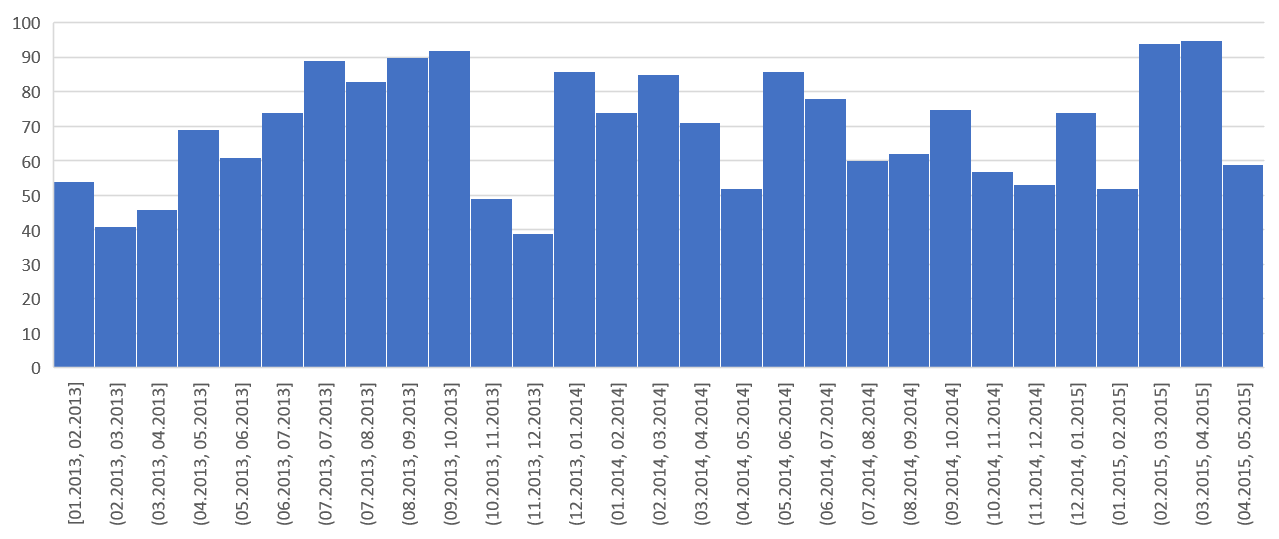
\includegraphics[width=0.8\textwidth]{Histo_Quote_Date.png}
	\end{center}
	\caption{Histogramm Quote\_Date}
\end{figure}


\subsubsection{Quote\_Flag}
\paragraph{Attribute type: nominal (dichotomous)}
The description of the attributes declares "Quote\_Flag" as information about whether an insurance was purchased. This can be only answered with yes or no.

\begin{table}[H]
	\renewcommand{\arraystretch}{1.25}
	\begin{tabular}{l|l}
		\textbf{Statistic} & \textbf{Value}\\\hline
		Missing Values& None\\\hline
	\end{tabular}
\end{table}

\begin{table}[H]
	\renewcommand{\arraystretch}{1.25}
		\begin{tabular}{l|l|l}
			\textbf{Value} & \textbf{Absolute Frequency} & \textbf{Relative Frequency}\\\hline
			0 & $1605$ & $0.8025$\\ \hline
			1 & $395$ & $0.1975$\\
		\end{tabular}
\end{table}

\begin{figure}[H]
	\begin{center}
		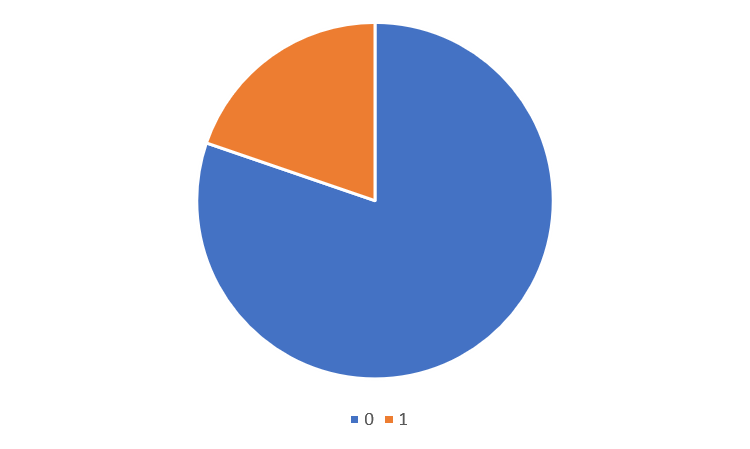
\includegraphics[width=0.8\textwidth]{Pie_Quote_Flag.png}
	\end{center}
	\caption{Pie Graph Quote\_Flag}
\end{figure}


\subsection{Field\_Info1}
\paragraph{Attribute type: nominal} These characters are not close enough together to asssume, they belong to a ordererd attribute.

\begin{table}[H]
	\renewcommand{\arraystretch}{1.25}
	\begin{tabular}{l|l}
		\textbf{Statistic} & \textbf{Value}\\\hline
		Missing Values& None\\\hline
	\end{tabular}
\end{table}


\begin{table}[H]
	\renewcommand{\arraystretch}{1.25}
	\begin{tabular}{l|l|l}
		\textbf{Value} & \textbf{Absolute Frequency} & \textbf{Relative Frequency}\\\hline
			J&$390$ & $0.365$\\\hline
			F&$540$ & $0.27$\\\hline
			B&$730$ & $0.195$\\\hline
			E&$200$ & $0.1$\\\hline
			C&$39$ & $0.0505$\\\hline
			K&$101$ & $0.0195$\\
	\end{tabular}
\end{table}

\begin{figure}[H]
	\begin{center}
		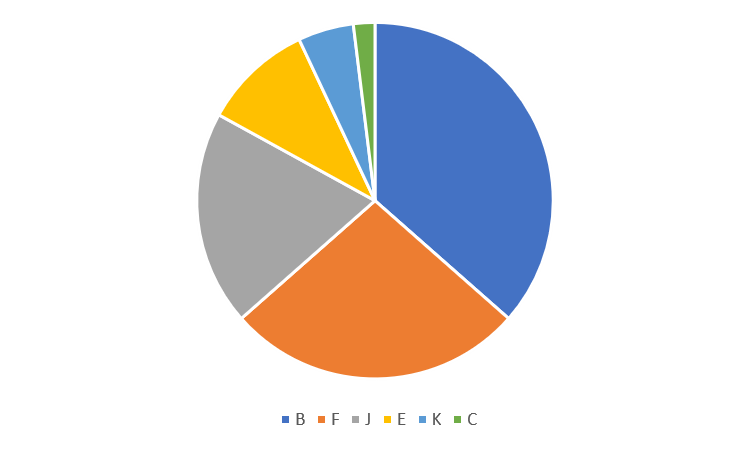
\includegraphics[width=0.8\textwidth]{Pie_Field_Info2.png}
	\end{center}
	\caption{Pie Graph Field\_Info1}
\end{figure}


\subsection{Field\_Info2}
\paragraph{Attribute type: ratio}
All values of "Field\_Info2" are numbers between $0$ and $2$ and have a precision of 4 decimals. This suggests that these values are on a zero-based scale.
\begin{table}[H]
	\renewcommand{\arraystretch}{1.25}
	\begin{tabular}{l|l}
		\textbf{Statistic} & \textbf{Value}\\\hline
			Missing Values& None\\\hline
			Minimum& $0.8746$\\\hline
			Maximum& $1.0101$\\\hline
			Mean& $0.9391$\\\hline
			Std. Dev.& $0.0373$\\\hline
			90th Perc. & $1.00051$\\\hline
			10th Perc. & $0.8922$ \\
	\end{tabular}
\end{table}

\begin{figure}[H]
	\begin{center}
		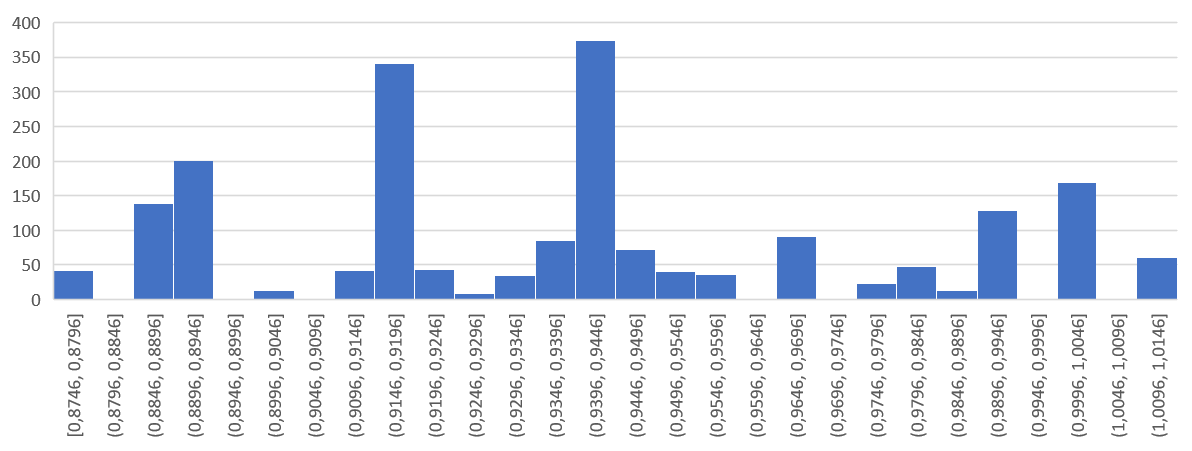
\includegraphics[width=0.8\textwidth]{Histo_Field_Info2.png}
	\end{center}
	\caption{Histogramm Field\_Info2}
\end{figure}

\subsection{Field\_Info3}
\paragraph{Attribute type: ratio} The values in this attribute are all numeric range in a range of around $1000$. Given the size of the numbers this could be a attribute containing monetary values.

\begin{table}[H]
	\renewcommand{\arraystretch}{1.25}
	\begin{tabular}{l|l}
		\textbf{Statistic} & \textbf{Value}\\\hline
			Missing Values& None\\\hline
		Minimum& $548$\\\hline
		Maximum& $1487$\\\hline
		Mean& $950.5195$\\\hline
		Std. Dev.& $290.62$\\\hline
		90th Perc. & $901480$\\\hline
		10th Perc. & $548$ \\		
	\end{tabular}
\end{table}

\begin{figure}[H]
	\begin{center}
		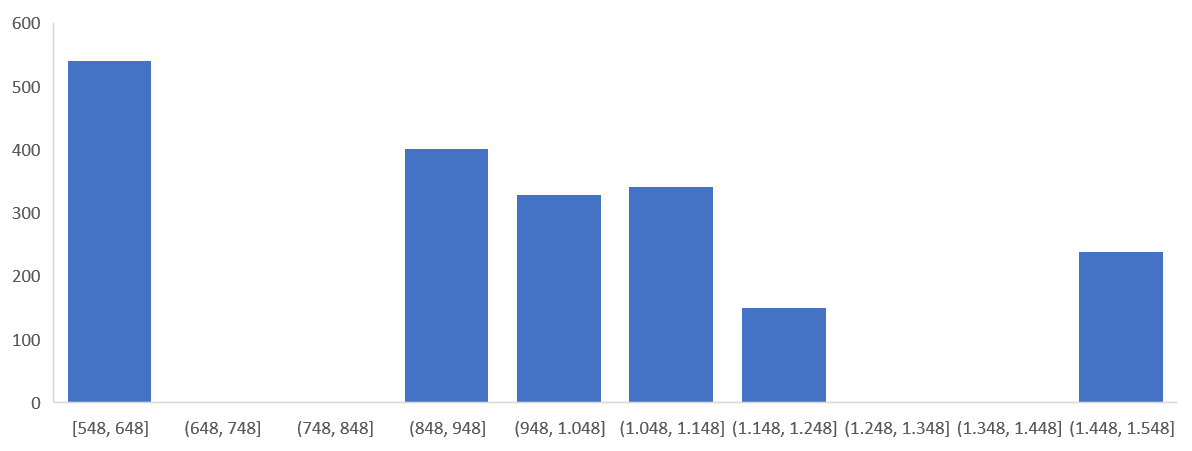
\includegraphics[width=0.8\textwidth]{Histo_Field_Info3.png}
	\end{center}
	\caption{Histogramm Field\_Info3}
\end{figure}

\subsection{Field\_Info4}
\paragraph{Attribute type: nominal (dichotomous)} In this Attribute only the values "Y" and "N" appear. Those values are often used as a short version on "Yes" and "No". This field therefore seems to be a yes-no answer.
\qquad
\begin{table}[H]
	\renewcommand{\arraystretch}{1.25}
	\begin{tabular}{l|l}
		\textbf{Statistic} & \textbf{Value}\\\hline
		Missing Values& None\\\hline
	\end{tabular}
\end{table}
\begin{table}[H]
	\renewcommand{\arraystretch}{1.25}
	\begin{tabular}{l|l|l}
		\textbf{Value} & \textbf{Absolute Frequency} & \textbf{Relative Frequency}\\\hline
		N	&$1860$&$0.93$\\\hline
		Y&	$140$&$0.07$
	\end{tabular}
\end{table}

\begin{figure}[H]
	\begin{center}
		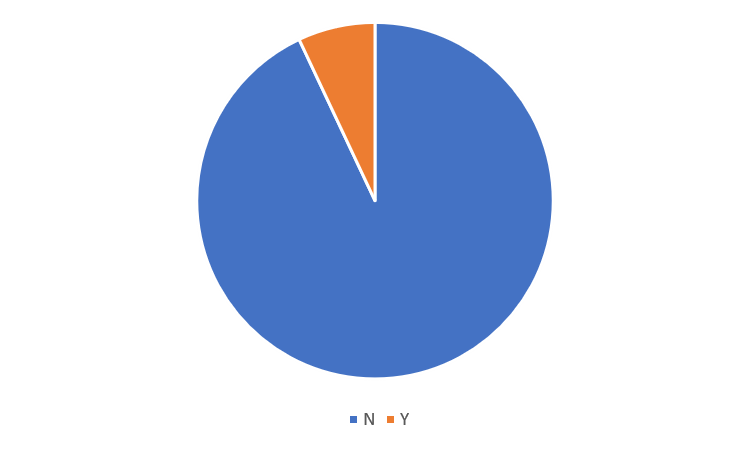
\includegraphics[width=0.8\textwidth]{Pie_Field_Info4.png}
	\end{center}
	\caption{Pie Graph Field\_Info4}
\end{figure}

\subsection{Coverage\_Info1}
\paragraph{Attribute type: ordinal} This attribute contains values from $1$ to $25$.  These could be different values in a specified order but not a numeric value.

\begin{table}[H]
	\renewcommand{\arraystretch}{1.25}
	\begin{tabular}{l|l}
		\textbf{Statistic} & \textbf{Value}\\\hline
		Missing Values& None\\\hline
		Numeric Outliers & $74$
	\end{tabular}
\end{table}

\begin{table}[H]
	\renewcommand{\arraystretch}{1.25}
	\begin{tabular}{l|l|l}
		\textbf{Value} & \textbf{Absolute Frequency} & \textbf{Relative Frequency}\\\hline
		-1&$2$&$0.001$\\\hline
		1&$42$&$0.021$\\\hline
		2&$81$&$0.0405$\\\hline
		3&$118$&$0.059$\\\hline
		4&$149$&$0.0745$\\\hline
		5&$189$&$0.0945$\\\hline
		6&$182$&$0.091$\\\hline
		7&$185$&$0.0925$\\\hline
		8&$148$&$0.074$\\\hline
		9&$151$&$0.0755$\\\hline
		10&$113$&$0.0565$\\\hline
		11&$106$&$0.053$\\\hline
		12&$83$&$0.0415$\\\hline
		13&$67$&$0.0335$\\\hline
		14&$62$&$0.031$\\\hline
		15&$53$&$0.0265$\\\hline
		16&$49$&$0.0245$\\\hline
		17&$35$&$0.0175$\\\hline
		18&$37$&$0.0185$\\\hline
		19&$19$&$0.0095$\\\hline
		20&$18$&$0.009$\\\hline
		21&$19$&$0.0095$\\\hline
		22&$18$&$0.009$\\\hline
		23&$12$&$0.006$\\\hline
		24&$11$&$0.0055$\\\hline
		25&$51$&$0.0255$
	\end{tabular}
\end{table}

\begin{figure}[H]
	\begin{center}
		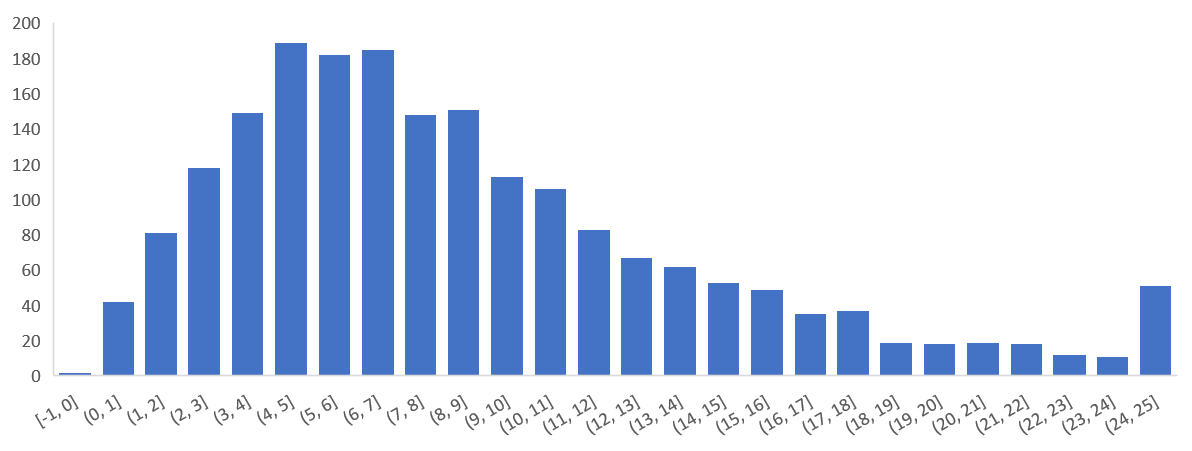
\includegraphics[width=0.8\textwidth]{Histo_Coverage_Info1.png}
	\end{center}
	\caption{Histogramm Coverage\_Info1}
\end{figure}

\subsection{Coverage\_Info2}
\paragraph{Attribute type: ordinal}As before, this attribute contains values from $1$ to $25$.  These could be different values in a specified order but not a numeric value but we only got datapoints with values at $1$,$2$, $22$ and $25$, which is quite interesting as only $3$ customers selected value $1$

\begin{table}[H]
	\renewcommand{\arraystretch}{1.25}
	\begin{tabular}{l|l}
		\textbf{Statistic} & \textbf{Value}\\\hline
		Missing Values& None\\\hline
	\end{tabular}
\end{table}
\begin{table}[H]
	\renewcommand{\arraystretch}{1.25}
	\begin{tabular}{l|l|l}
		\textbf{Value} & \textbf{Absolute Frequency} & \textbf{Relative Frequency}\\\hline
		1&$3$&$0.0015$\\\hline
		2&$125$&$0.0625$\\\hline
		22&$1620$&$0.81$\\\hline
		25&$252$&$0.126$\\\hline
	\end{tabular}
\end{table}

\begin{figure}[H]
	\begin{center}
		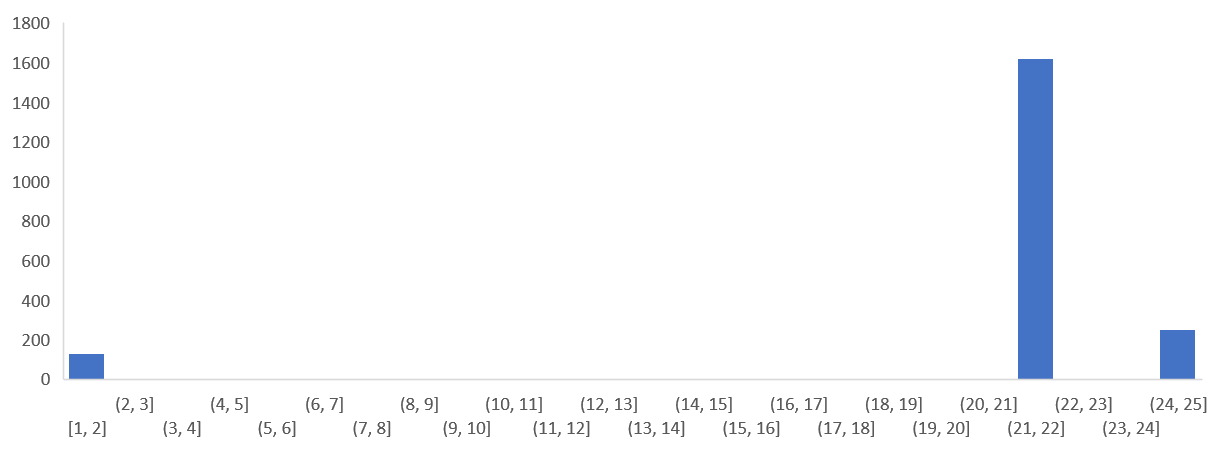
\includegraphics[width=0.8\textwidth]{Histo_Coverage_Info2.png}
	\end{center}
	\caption{Histogramm Coverage\_Info2}
\end{figure}

\subsection{Coverage\_Info3}
\paragraph{Attribute type: ordinal} This field contains letters from the beginning of the alphabet. This indicates for these values to be ordered in that order.

\begin{table}[H]
	\renewcommand{\arraystretch}{1.25}
	\begin{tabular}{l|l}
		\textbf{Statistic} & \textbf{Value}\\\hline
		Missing Values& None\\\hline
	\end{tabular}
\end{table}
\begin{table}[H]
	\renewcommand{\arraystretch}{1.25}
	\begin{tabular}{l|l|l}
		\textbf{Value} & \textbf{Absolute Frequency} & \textbf{Relative Frequency}\\\hline
		A&$116$&$0.058$\\\hline
		B&$4$&$0.002$\\\hline
		C&$3$&$0.0015$\\\hline
		D&$388$&$0.194$\\\hline
		E&$673$&$0.3365$\\\hline
		F&$221$&$0.1105$\\\hline
		G&$245$&$0.1225$\\\hline
		H&$2$&$0.001$\\\hline
		I&$7$&$0.0035$\\\hline
		J&$110$&$0.055$\\\hline
		K&$229$&$0.1145$\\\hline
		L&$2$&$0.001$
	\end{tabular}
\end{table}
\begin{figure}[H]
	\begin{center}
		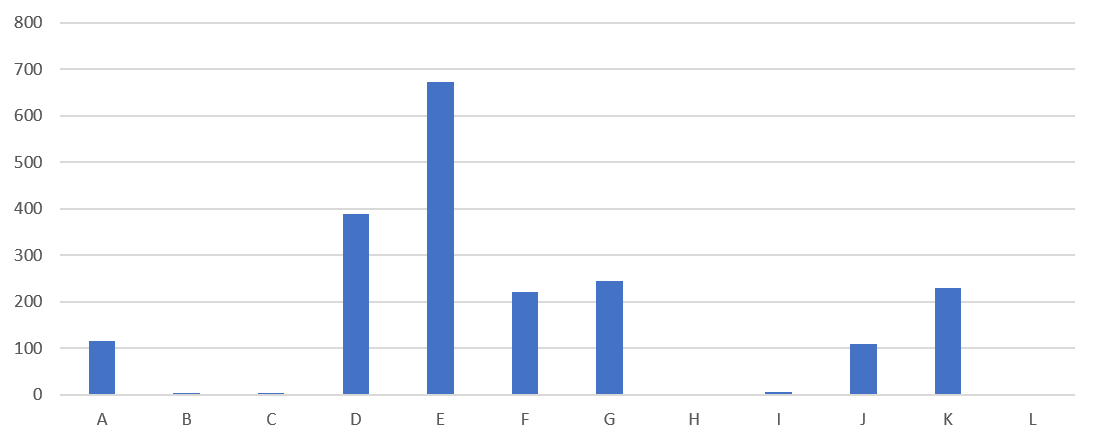
\includegraphics[width=0.8\textwidth]{Histo_Coverage_Info3.png}
	\end{center}
	\caption{Histogramm Coverage\_Info3}
\end{figure}

\subsection{Sales\_Info1}
\paragraph{Attribute type: nominal (dichotomous)}
\qquad
\begin{table}[H]
	\renewcommand{\arraystretch}{1.25}
	\begin{tabular}{l|l}
		\textbf{Statistic} & \textbf{Value}\\\hline
		Missing Values& None\\\hline
	\end{tabular}
\end{table}
\begin{table}[H]
	\renewcommand{\arraystretch}{1.25}
	\begin{tabular}{l|l|l}
		\textbf{Value} & \textbf{Absolute Frequency} & \textbf{Relative Frequency}\\\hline
		1&$1490$&$0.745$\\\hline
		0&$510$&$0.255$
	\end{tabular}
\end{table}
\begin{figure}[H]
	\begin{center}
		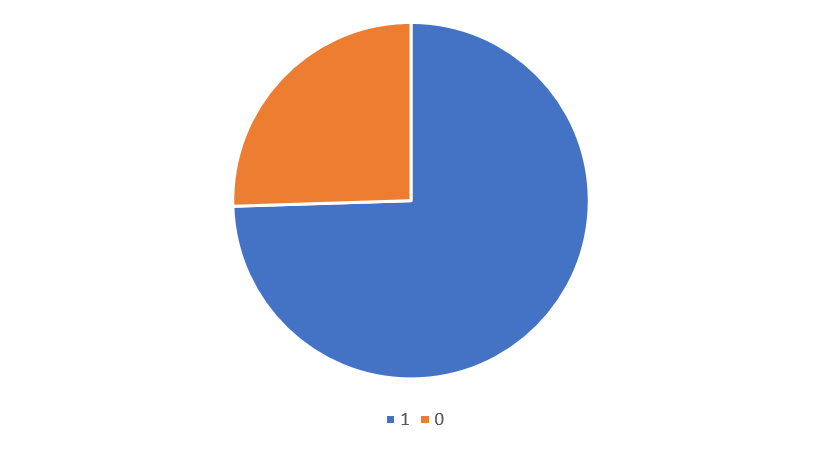
\includegraphics[width=0.8\textwidth]{Pie_Sales_Info1.png}
	\end{center}
	\caption{Pie Graph Sales\_Info1}
\end{figure}

\subsection{Sales\_Info2}
\paragraph{Attribute type: ordinal} This Attributes contains numbers from $2$ to $5$. Probably, the provided data is missing the value $1$. With that value these could be values ordered from $1$ to $5$.
\qquad
\begin{table}[H]
	\renewcommand{\arraystretch}{1.25}
	\begin{tabular}{l|l}
		\textbf{Statistic} & \textbf{Value}\\\hline
		Missing Values& None\\\hline
	\end{tabular}
\end{table}
\begin{table}[H]
	\renewcommand{\arraystretch}{1.25}
	\begin{tabular}{l|l|l}
		\textbf{Value} & \textbf{Absolute Frequency} & \textbf{Relative Frequency}\\\hline
		2&$93$&$0.0465$\\\hline
		3&$519$&$0.2595$\\\hline
		4&$295$&$0.1475$\\\hline
		5&$1093$&$0.5465$
	\end{tabular}
\end{table}
\begin{figure}[H]
	\begin{center}
		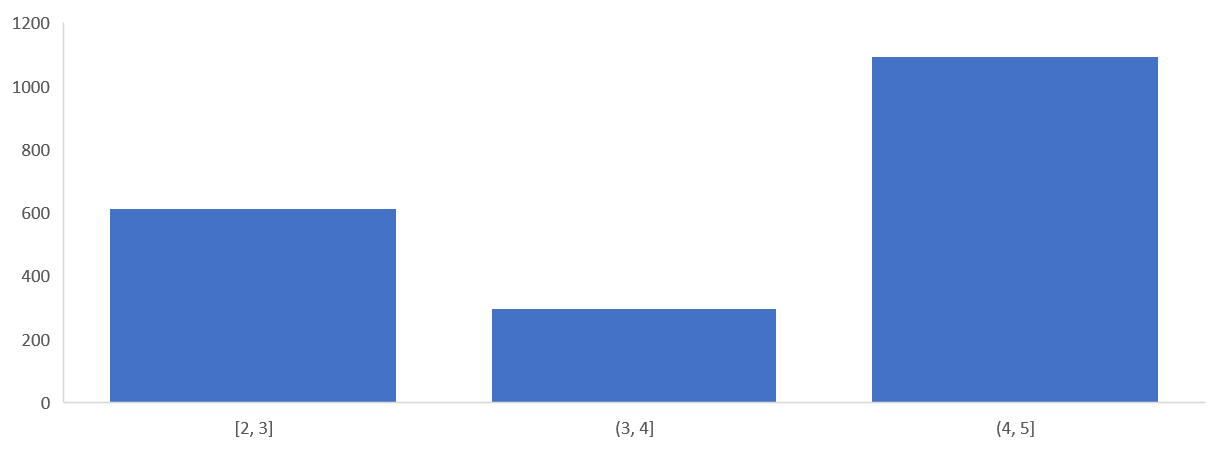
\includegraphics[width=0.8\textwidth]{Histo_Sales_Info2.png}
	\end{center}
	\caption{Histogramm Sales\_Info2}
\end{figure}

\subsection{Sales\_Info3}
\paragraph{Attribute type: ordinal} Like Coverage\_Info1 this is a ordinal attribute, but we are missing some values inside the provided range.

\qquad
\begin{table}[H]
	\renewcommand{\arraystretch}{1.25}
	\begin{tabular}{l|l}
		\textbf{Statistic} & \textbf{Value}\\\hline
		Missing Values& None\\\hline
	\end{tabular}
\end{table}
\begin{figure}[H]
	\begin{center}
		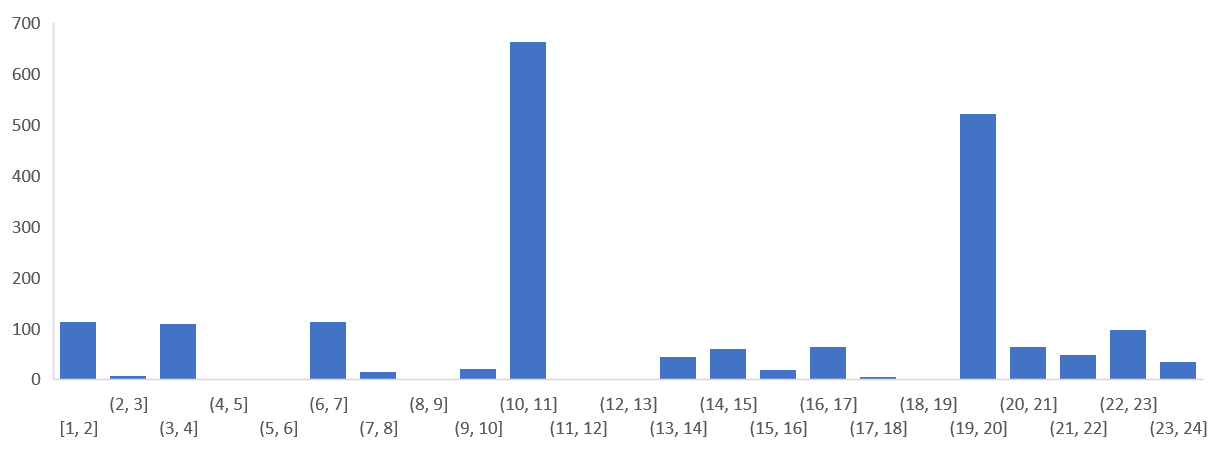
\includegraphics[width=0.8\textwidth]{Histo_Sales_Info3.png}
	\end{center}
	\caption{Histogramm Sales\_Info3}
\end{figure}

\subsection{Sales\_Info4}
\paragraph{Attribute type: nominal} These letters seem to have no recognisable order.

\begin{table}[H]
	\renewcommand{\arraystretch}{1.25}
	\begin{tabular}{l|l}
		\textbf{Statistic} & \textbf{Value}\\\hline
		Missing Values& None\\\hline
	\end{tabular}
\end{table}
\begin{table}[H]
	\renewcommand{\arraystretch}{1.25}
	\begin{tabular}{l|l|l}
		\textbf{Value} & \textbf{Absolute Frequency} & \textbf{Relative Frequency}\\\hline
		K&$410$&$0.205$\\\hline
		P&$376$&$0.188$\\\hline
		T&$332$&$0.166$\\\hline
		Q&$312$&$0.156$\\\hline
		V&$298$&$0.149$\\\hline
		R&$156$&$0.078$\\\hline
		M&$116$&$0.058$
	\end{tabular}
\end{table}

\begin{figure}[H]
	\begin{center}
		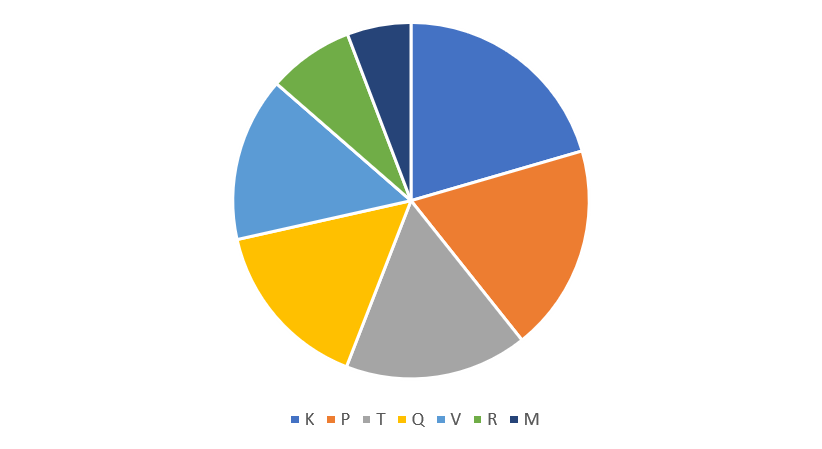
\includegraphics[width=0.8\textwidth]{Pie_Sales_Info4.png}
	\end{center}
	\caption{Pie Graph Sales\_Info4}
\end{figure}

\subsection{Sales\_Info5}
\paragraph{Attribute type: ratio} The values in this attribute are distributed very evenly and range in a big range. Given the size of the numbers this could be a attribute containing monetary values.

\begin{table}[H]
	\renewcommand{\arraystretch}{1.25}
	\begin{tabular}{l|l}
		\textbf{Statistic} & \textbf{Value}\\\hline
		Missing Values& None\\\hline
		Minimum& $1$\\\hline
		Maximum& $67162$\\\hline
		Mean& $33785.54$\\\hline
		Std. Dev.& $18863.43$\\\hline
		90th Perc. & $59741.7$\\\hline
		10th Perc. & $7828.9$ \\		
	\end{tabular}
\end{table}
\begin{figure}[H]
	\begin{center}
		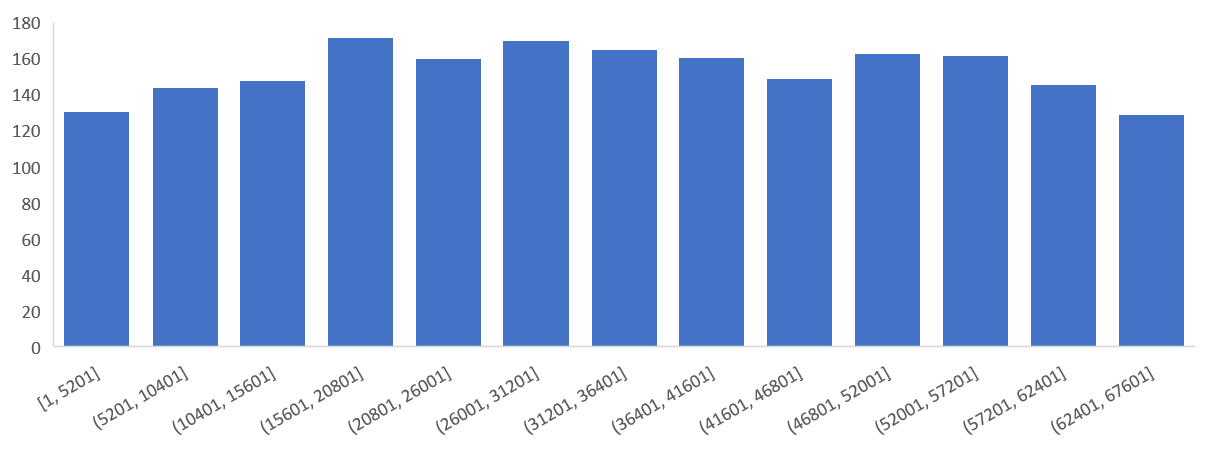
\includegraphics[width=0.8\textwidth]{Histo_Sales_Info5.png}
	\end{center}
	\caption{Histogramm Sales\_Info5}
\end{figure}

\subsection{Personal\_Info1}
\paragraph{Attribute type: nominal (dichotomous)}\quad

\begin{table}[H]
	\renewcommand{\arraystretch}{1.25}
	\begin{tabular}{l|l}
		\textbf{Statistic} & \textbf{Value}\\\hline
		Missing Values& None\\\hline
	\end{tabular}
\end{table}
\begin{table}[H]
	\renewcommand{\arraystretch}{1.25}
	\begin{tabular}{l|l|l}
		\textbf{Value} & \textbf{Absolute Frequency} & \textbf{Relative Frequency}\\\hline
		N&$1993$&$0.9965$\\\hline
		Y&$7$&$0.0035$
	\end{tabular}
\end{table}

\begin{figure}[H]
	\begin{center}
		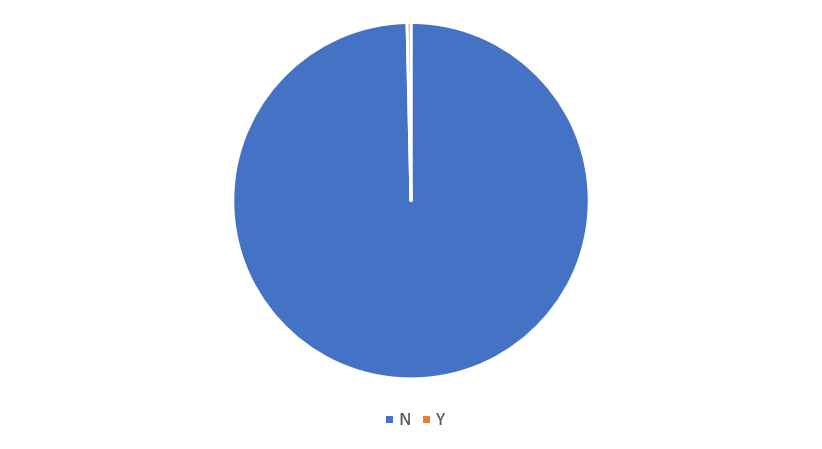
\includegraphics[width=0.8\textwidth]{Pie_Personal_Info1.png}
	\end{center}
	\caption{Pie Graph Personal\_Info1}
\end{figure}

\subsection{Personal\_Info2}
\paragraph{Attribute type: ordinal} Like Coverage\_Info1, this attribute probably also contains ordered values, but in the range between $1$ and $25$. And the value $-1$ means "no answer". 

\begin{table}[H]
	\renewcommand{\arraystretch}{1.25}
	\begin{tabular}{l|l}
		\textbf{Statistic} & \textbf{Value}\\\hline
		Missing Values& None\\\hline
	\end{tabular}
\end{table}
\begin{figure}[H]
	\begin{center}
		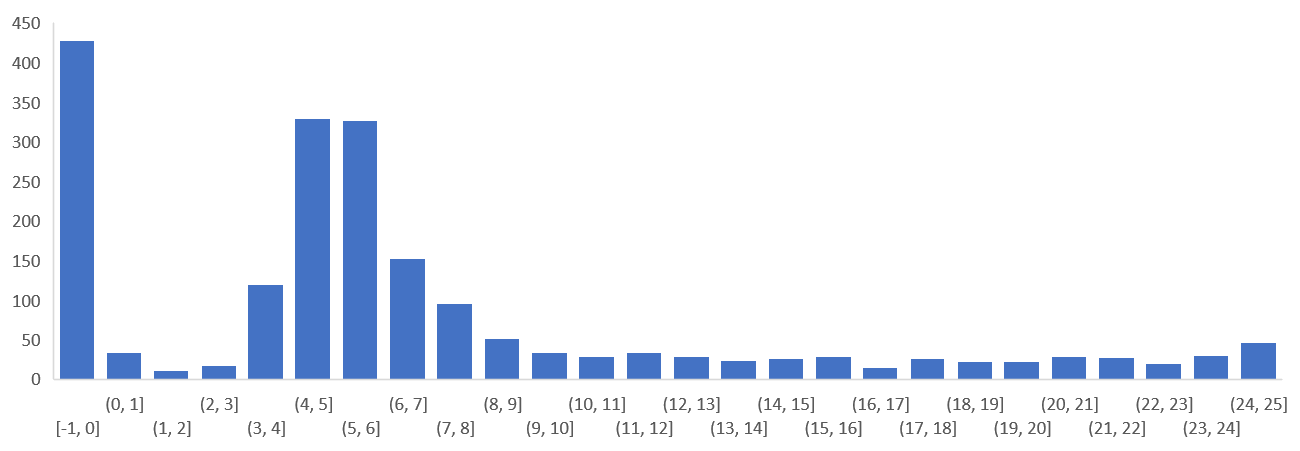
\includegraphics[width=0.8\textwidth]{Histo_Personal_Info2.png}
	\end{center}
	\caption{Histogramm Personal\_Info2}
\end{figure}

\subsection{Personal\_Info3}
\paragraph{Attribute type: nominal} These two letter combinations could be order in a alphabetic order, but they seem to start at a random place inside the alphabet. Therefore this attribute will be treated as nominal.

\begin{table}[H]
	\renewcommand{\arraystretch}{1.25}
	\begin{tabular}{l|l}
		\textbf{Statistic} & \textbf{Value}\\\hline
		Missing Values& None\\\hline
	\end{tabular}
\end{table}
\begin{table}[H]
	\renewcommand{\arraystretch}{1.25}
	\begin{tabular}{l|l|l}
		\textbf{Value} & \textbf{Absolute Frequency} & \textbf{Relative Frequency}\\\hline
		ZA&$937$&$0.4685$\\\hline
		XR&$104$&$0.052$\\\hline
		XM&$81$&$0.0405$\\\hline
		XJ&$73$&$0.0365$\\\hline
		XD&$63$&$0.0315$\\\hline
		XX&$62$&$0.031$\\\hline
		XB&$59$&$0.0295$\\\hline
		YH&$58$&$0.029$\\\hline
		XH&$54$&$0.027$\\\hline
		ZT&$51$&$0.0255$\\\hline
		XO&$50$&$0.025$\\\hline
		ZF&$46$&$0.023$\\\hline
		ZR&$40$&$0.02$\\\hline
		ZN&$39$&$0.0195$\\\hline
		ZH&$37$&$0.0185$\\\hline
		XS&$35$&$0.0175$\\\hline
		YF&$29$&$0.0145$\\\hline
		XW&$23$&$0.0115$\\\hline
		ZG&$20$&$0.01$\\\hline
		XE&$20$&$0.01$\\\hline
		ZW&$18$&$0.009$\\\hline
		YE&$17$&$0.0085$\\\hline
		ZC&$16$&$0.008$\\\hline
		XC&$14$&$0.007$\\\hline
		XQ&$14$&$0.007$\\\hline
		XL&$7$&$0.0035$\\\hline
		ZE&$7$&$0.0035$\\\hline
		ZJ&$6$&$0.003$\\\hline
		XI&$5$&$0.0025$\\\hline
		ZD&$5$&$0.0025$\\\hline
		ZK&$4$&$0.002$\\\hline
		XZ&$4$&$0.002$\\\hline
		ZU&$2$&$0.001$
	\end{tabular}
\end{table}

\begin{figure}[H]
	\begin{center}
		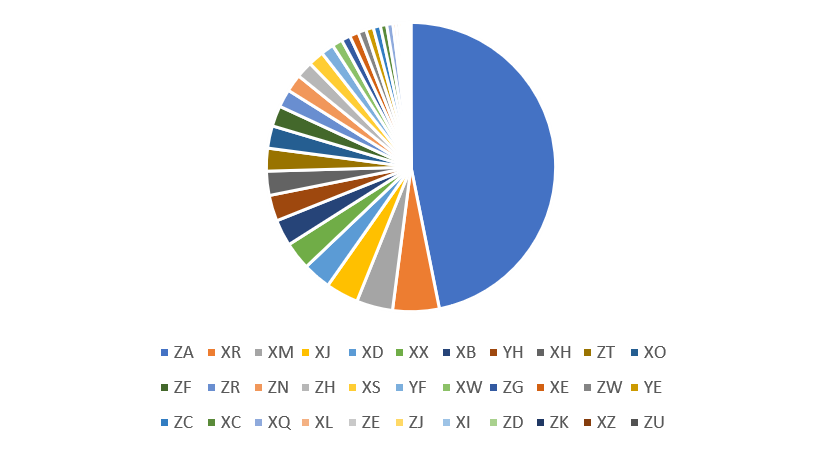
\includegraphics[width=0.8\textwidth]{Pie_Personal_Info3.png}
	\end{center}
	\caption{Pie Graph Personal\_Info3}
\end{figure}

\subsection{Personal\_Info4}
\paragraph{Attribute type: nominal (dichotomous)} \quad All those values are $0$ except for one, which is $1$.

\begin{table}[H]
	\renewcommand{\arraystretch}{1.25}
	\begin{tabular}{l|l}
		\textbf{Statistic} & \textbf{Value}\\\hline
		Missing Values& None\\\hline
		Outliers & $1$
	\end{tabular}
\end{table}
\begin{table}[H]
	\renewcommand{\arraystretch}{1.25}
	\begin{tabular}{l|l|l}
		\textbf{Value} & \textbf{Absolute Frequency} & \textbf{Relative Frequency}\\\hline
		0&$1999$&$0.9995$\\\hline
		1&$1$&$0.001$
	\end{tabular}
\end{table}


\subsection{Personal\_Info5}
\paragraph{Attribute type: ordinal}This Attribute has no value in a lot of Cases. This Attribute could have up to 5 different, ordered values ($1$ - $5$). This Attribute will probably not get looked at during prediction analysis.

\begin{table}[H]
	\renewcommand{\arraystretch}{1.25}
	\begin{tabular}{l|l}
		\textbf{Statistic} & \textbf{Value}\\\hline
		Missing Values& $966$\\\hline
	\end{tabular}
\end{table}

\subsection{Property\_Info1}
\paragraph{Attribute type: nominal (dichotomous)}
\begin{table}[H]
	\renewcommand{\arraystretch}{1.25}
	\begin{tabular}{l|l}
		\textbf{Statistic} & \textbf{Value}\\\hline
		Missing Values& $1$\\\hline
	\end{tabular}
\end{table}
\begin{table}[H]
	\renewcommand{\arraystretch}{1.25}
	\begin{tabular}{l|l|l}
		\textbf{Value} & \textbf{Absolute Frequency} & \textbf{Relative Frequency}\\\hline
		N&$1738$&$0.869$\\\hline
		Y&$261$&$0.1305$
\end{tabular}
\end{table}

\begin{figure}[H]
	\begin{center}
		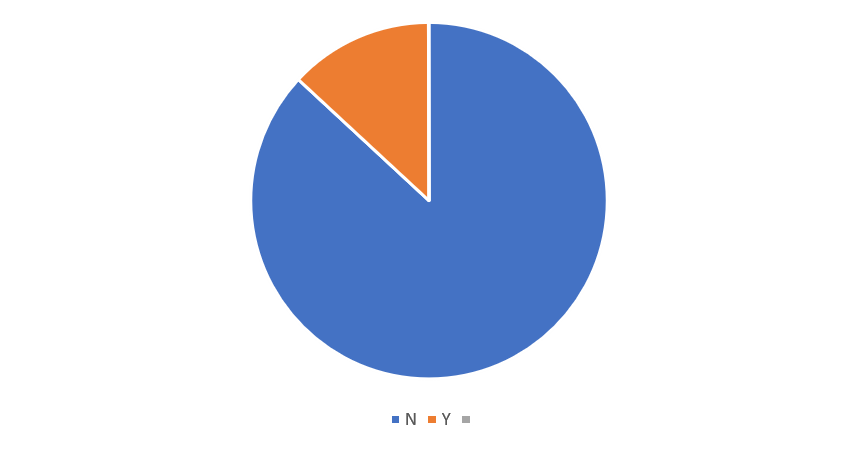
\includegraphics[width=0.8\textwidth]{Pie_Property_Info1.png}
	\end{center}
	\caption{Pie Graph Property\_Info1}
\end{figure}

\subsection{Property\_Info2}
\paragraph{Attribute type: nominal} All those values are $0$

\begin{table}[H]
	\renewcommand{\arraystretch}{1.25}
	\begin{tabular}{l|l}
		\textbf{Statistic} & \textbf{Value}\\\hline
		Missing Values& None\\\hline
	\end{tabular}
\end{table}


\subsection{Property\_Info3}
\paragraph{Attribute type: nominal} random letters

\begin{table}[H]
	\renewcommand{\arraystretch}{1.25}
	\begin{tabular}{l|l}
		\textbf{Statistic} & \textbf{Value}\\\hline
		Missing Values& None\\\hline
	\end{tabular}
\end{table}
\begin{table}[H]
	\renewcommand{\arraystretch}{1.25}
	\begin{tabular}{l|l|l}
		\textbf{Value} & \textbf{Absolute Frequency} & \textbf{Relative Frequency}\\\hline
		O&$573$&$0.2865$\\\hline
		R&$533$&$0.2665$\\\hline
		J&$285$&$0.1425$\\\hline
		D&$198$&$0.099$\\\hline
		S&$146$&$0.073$\\\hline
		N&$92$&$0.046$\\\hline
		I&$77$&$0.0385$\\\hline
		A&$31$&$0.0155$\\\hline
		Q&$30$&$0.015$\\\hline
		E&$10$&$0.005$\\\hline
		H&$9$&$0.0045$\\\hline
		K&$6$&$0.003$\\\hline
		F&$5$&$0.0025$\\\hline
		L&$3$&$0.0015$\\\hline
		G&$2$&$0.001$
	\end{tabular}
\end{table}
\begin{figure}[H]
	\begin{center}
		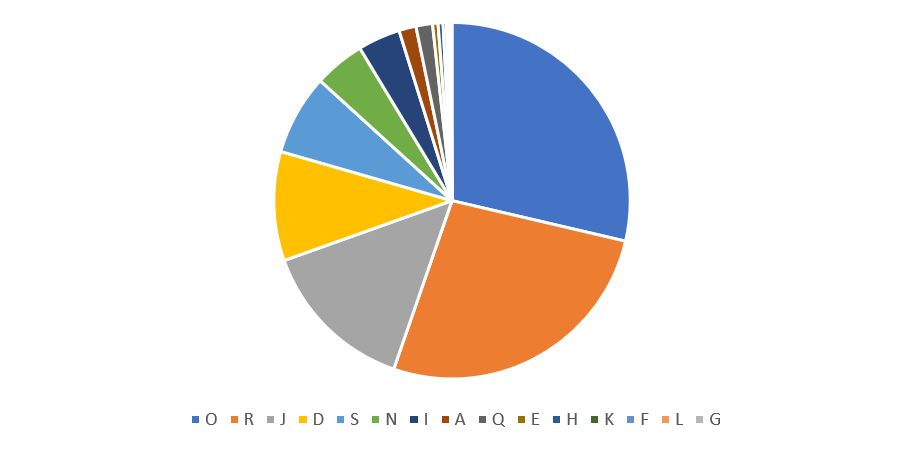
\includegraphics[width=0.8\textwidth]{Pie_Property_Info3.png}
	\end{center}
	\caption{Pie Graph Property\_Info3}
\end{figure}

\subsection{Property\_Info4}
\paragraph{Attribute type: nominal (dichotomous)}

\begin{table}[H]
	\renewcommand{\arraystretch}{1.25}
	\begin{tabular}{l|l}
		\textbf{Statistic} & \textbf{Value}\\\hline
		Missing Values& None\\\hline
	\end{tabular}
\end{table}
\begin{table}[H]
	\renewcommand{\arraystretch}{1.25}
	\begin{tabular}{l|l|l}
		\textbf{Value} & \textbf{Absolute Frequency} & \textbf{Relative Frequency}\\\hline
		1&$1364$&$0.682$\\\hline
		0&$636$&$0.318$
	\end{tabular}
\end{table}
\begin{figure}[H]
	\begin{center}
		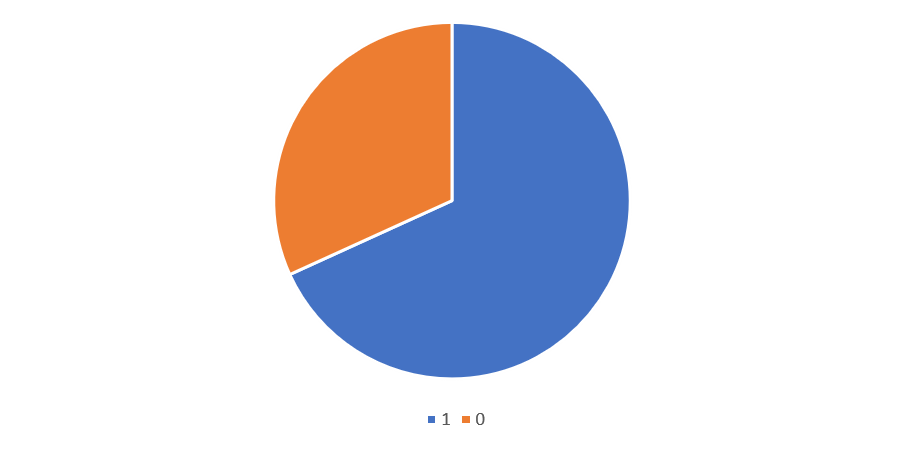
\includegraphics[width=0.8\textwidth]{Pie_Property_Info4.png}
	\end{center}
	\caption{Pie Graph Property\_Info4}
\end{figure}

\subsection{Property\_Info5}
\paragraph{Attribute type: ordinal} This Attribute too contains values from $1$ to $25$. I defined those as ordinal before.

\begin{table}[H]
	\renewcommand{\arraystretch}{1.25}
	\begin{tabular}{l|l}
		\textbf{Statistic} & \textbf{Value}\\\hline
		Missing Values& None\\\hline
	\end{tabular}
\end{table}

\begin{figure}[H]
	\begin{center}
		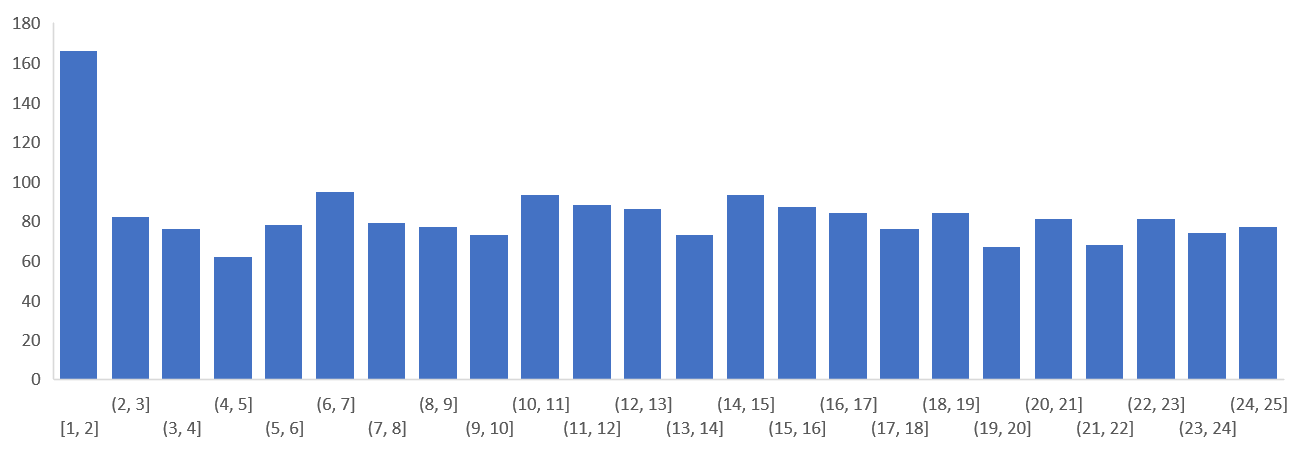
\includegraphics[width=0.8\textwidth]{Histo_Property_Info5.png}
	\end{center}
	\caption{Histogramm Property\_Info5}
\end{figure}

\subsection{Geographic\_Info1}
\paragraph{Attribute type: ordinal} This Attribute too contains values from $1$ to $25$. I defined those as ordinal before.

\begin{table}[H]
	\renewcommand{\arraystretch}{1.25}
	\begin{tabular}{l|l}
		\textbf{Statistic} & \textbf{Value}\\\hline
		Missing Values& None\\\hline
		Ouliers & 58
	\end{tabular}
\end{table}

\begin{figure}[H]
	\begin{center}
		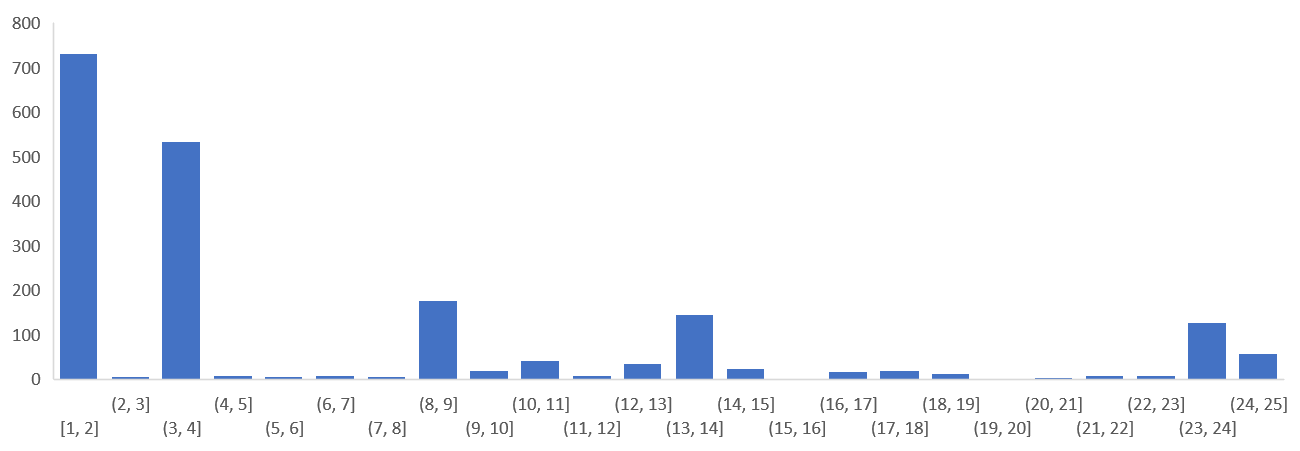
\includegraphics[width=0.8\textwidth]{Histo_Geographic_Info1.png}
	\end{center}
	\caption{Histogramm Geographic\_Info1}
\end{figure}

\subsection{Geographic\_Info2}
\paragraph{Attribute type: ordinal} This Attribute too contains values from $1$ to $25$. I defined those as ordinal before.

\begin{table}[H]
	\renewcommand{\arraystretch}{1.25}
	\begin{tabular}{l|l}
		\textbf{Statistic} & \textbf{Value}\\\hline
		Missing Values& None\\\hline		
	\end{tabular}
\end{table}

\begin{figure}[H]
	\begin{center}
		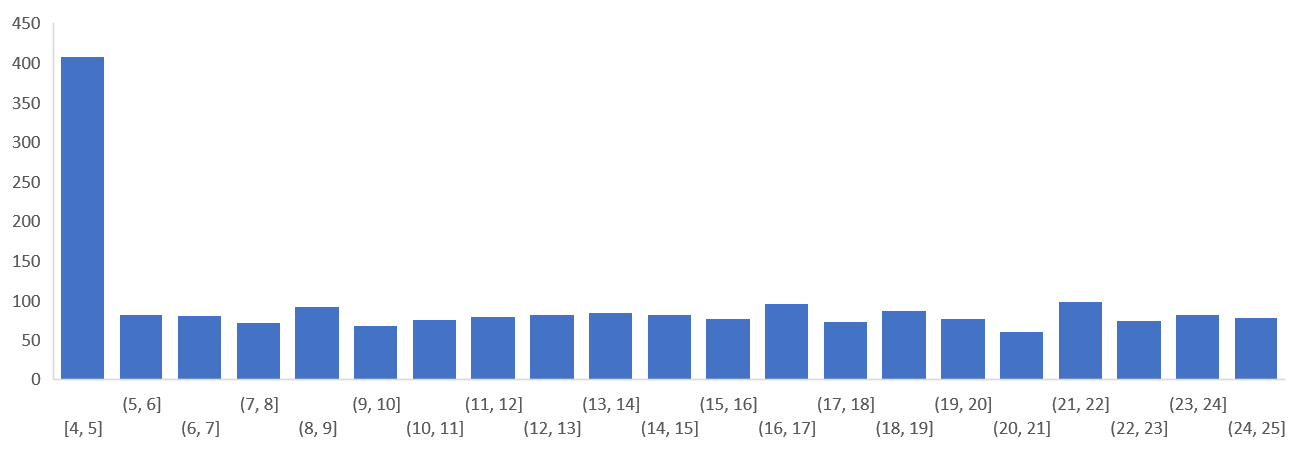
\includegraphics[width=0.8\textwidth]{Histo_Geographic_Info2.png}
	\end{center}
	\caption{Histogramm Geographic\_Info2}
\end{figure}

\subsection{Geographic\_Info3}
\paragraph{Attribute type: nominal} These values are very interessting. They could belong to a ordered attribute like "Personal\_Info2". Nevertheless, it is defined as nominal because too many values are missing.

\begin{table}[H]
	\renewcommand{\arraystretch}{1.25}
	\begin{tabular}{l|l}
		\textbf{Statistic} & \textbf{Value}\\\hline
		Missing Values& None\\\hline
	\end{tabular}
\end{table}
\begin{table}[H]
	\renewcommand{\arraystretch}{1.25}
	\begin{tabular}{l|l|l}
		\textbf{Value} & \textbf{Absolute Frequency} & \textbf{Relative Frequency}\\\hline
		-1&$1942$&$0.971$\\\hline
		25&$58$&$0.029$
	\end{tabular}
\end{table}

\subsection{Geographic\_Info4}
\paragraph{Attribute type: nominal (dichotomous)}\quad

\begin{table}[H]
	\renewcommand{\arraystretch}{1.25}
	\begin{tabular}{l|l}
		\textbf{Statistic} & \textbf{Value}\\\hline
		Missing Values& None\\\hline
	\end{tabular}
\end{table}
\begin{table}[H]
	\renewcommand{\arraystretch}{1.25}
	\begin{tabular}{l|l|l}
		\textbf{Value} & \textbf{Absolute Frequency} & \textbf{Relative Frequency}\\\hline
		N&$1961$&$0.9805$\\\hline
		Y&$39$&$0.0195$
	\end{tabular}
\end{table}
\begin{figure}[H]
	\begin{center}
		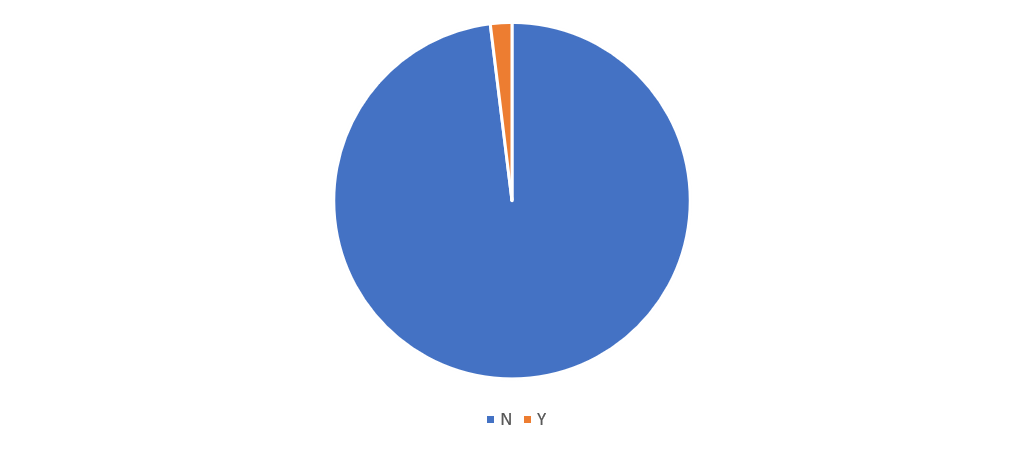
\includegraphics[width=0.8\textwidth]{Pie_Geographic_Info4.png}
	\end{center}
	\caption{Pie Graph Geographic\_Info4}
\end{figure}

\subsection{Geographic\_Info5}
\paragraph{Attribute type: nominal} These values could be the states California, New Jersey, Texas and Illinois. They also could represent any other value and don't have any specific order.

\begin{table}[H]
	\renewcommand{\arraystretch}{1.25}
	\begin{tabular}{l|l}
		\textbf{Statistic} & \textbf{Value}\\\hline
		Missing Values& None\\\hline
	\end{tabular}
\end{table}
\begin{table}[H]
	\renewcommand{\arraystretch}{1.25}
	\begin{tabular}{l|l|l}
		\textbf{Value} & \textbf{Absolute Frequency} & \textbf{Relative Frequency}\\\hline
		CA&$730$&$0.365$\\\hline
		NJ&$540$&$0.27$\\\hline
		TX&$491$&$0.2455$\\\hline
		IL&$239$&$0.1195$
	\end{tabular}
\end{table}

\begin{figure}[H]
	\begin{center}
		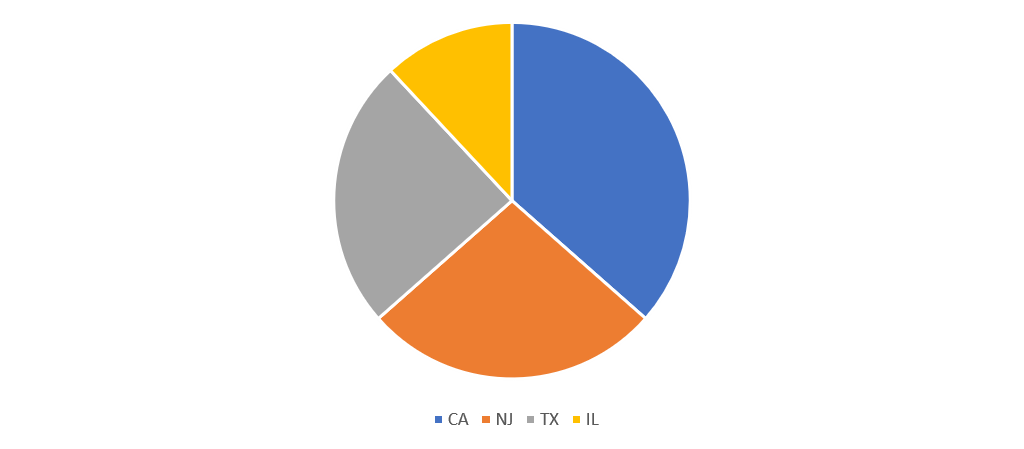
\includegraphics[width=0.8\textwidth]{Pie_Geographic_Info5.png}
	\end{center}
	\caption{Pie Graph Geographic\_Info5}
\end{figure}

\subsection{Interesting Attributes}

\paragraph{Field\_Info3} All values in this attribute are either on the side or in the middle of the range. 

\paragraph{Field\_Info4} Normal distribution, but there is a peak at the end.

\paragraph{Coverage\_Info2} On this attribute we only have datapoints with four different values allthough the range of those values suggets 25 options have been available.

\paragraph{Geographic\_Info2 \& Property\_Info 5} Both of these values show a  even distribution with a spike at the begin of their ranges.

\paragraph{Personal\_Info3} Almost $50 \text{\%}$ of the values are "ZA".
\paragraph{Property\_Info2} All values are $0$
\paragraph{Personal\_Info4} All values are $0$ except for one $1$

\subsubsection{Linear Correlations}

There are some interessting correlations in this dataset. Exspecially Geographic\_Info5 seems to have some strong correllations with Field\_Info2 and Coverage\_Info3. Field\_Info1 seems to be correlatted to Field\_Info4 and Field\_Info2 has as negative Correlation with Field\_Info3.

\begin{figure}[H]
	\begin{center}
		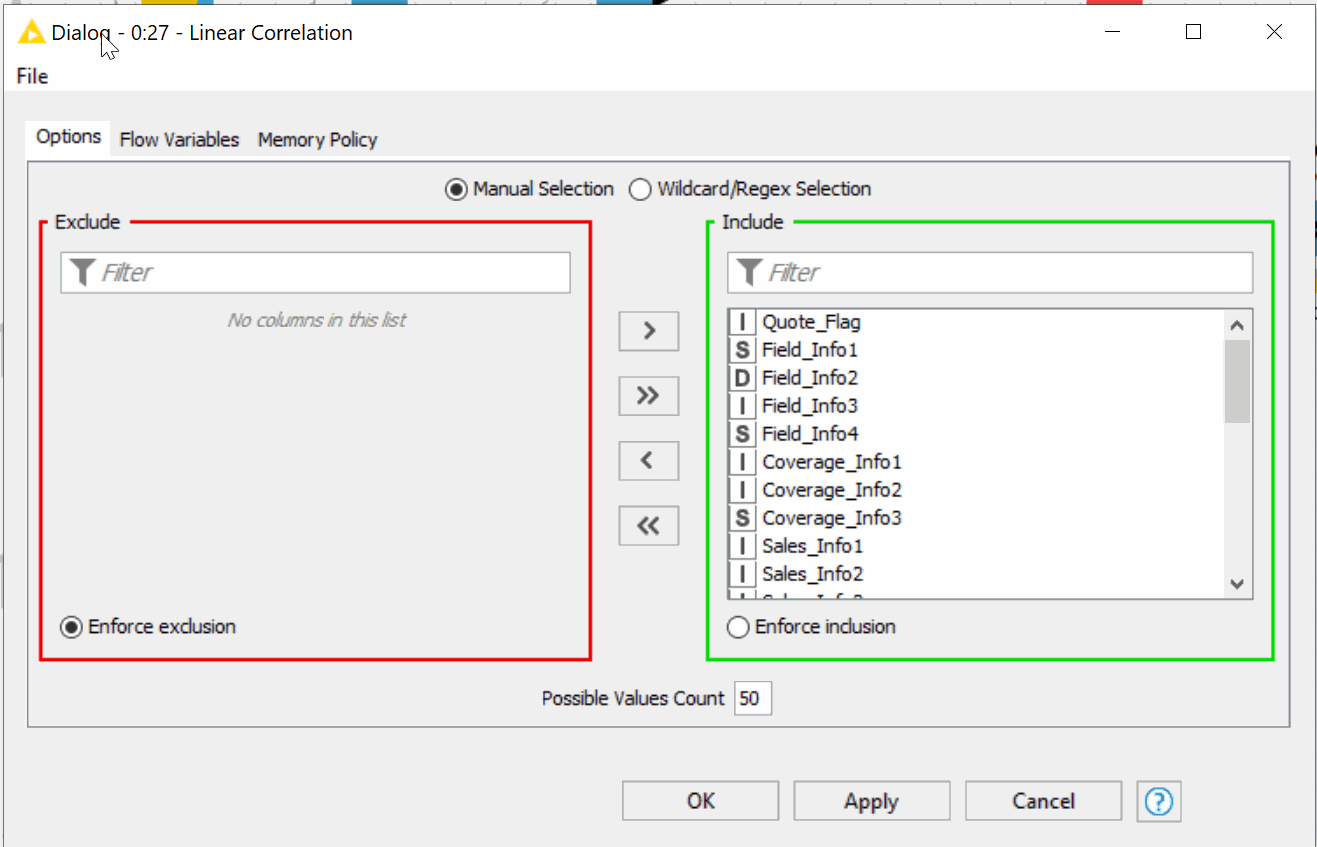
\includegraphics[width=0.4\textwidth]{Screen/Screen_Corr_1.png}
		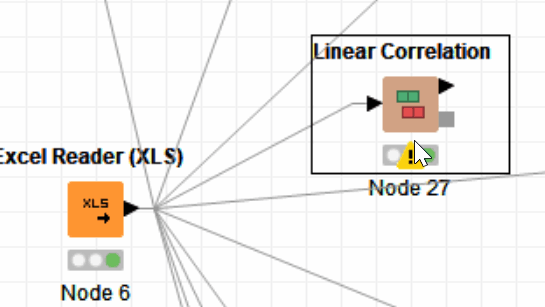
\includegraphics[width=0.4\textwidth]{Screen/Screen_Corr_3.png}
		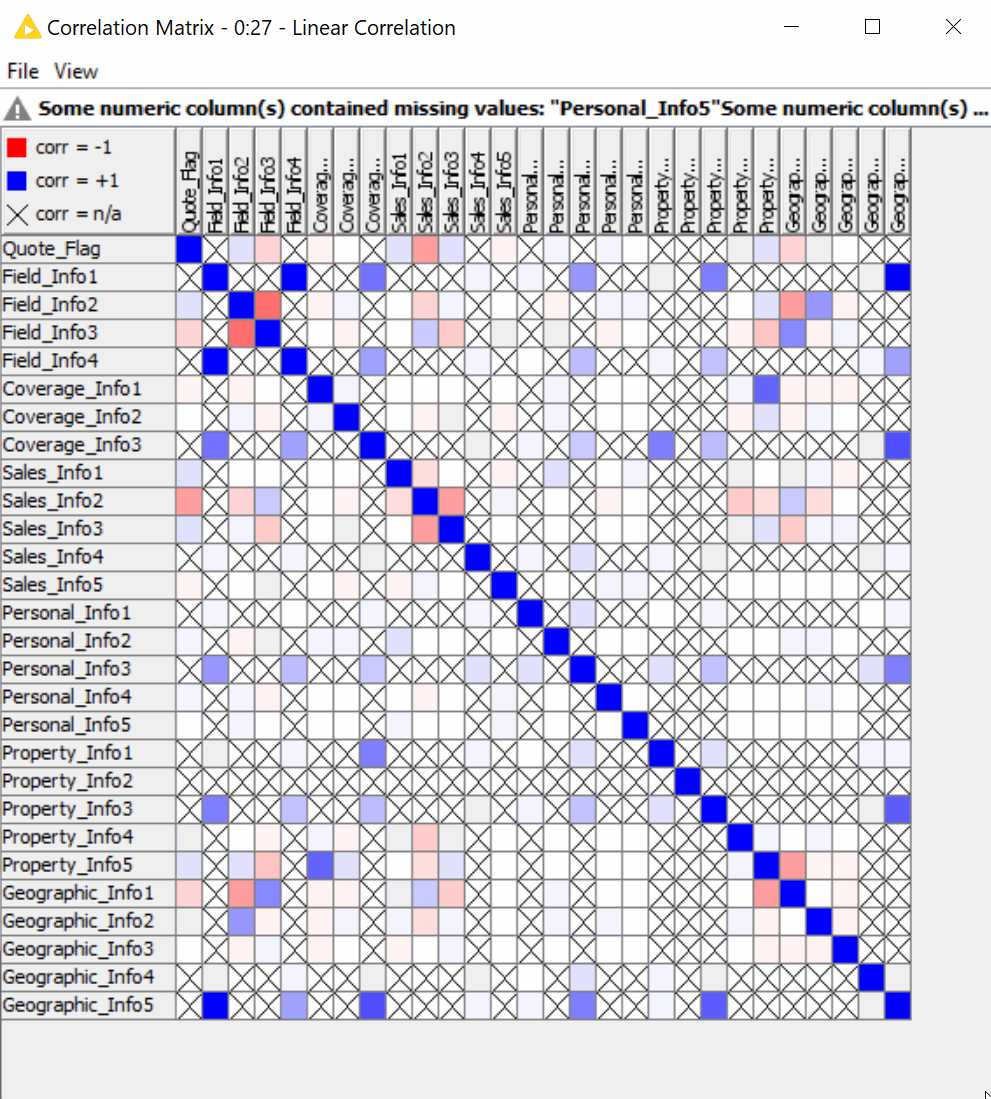
\includegraphics[width=0.4\textwidth]{Screen/Screen_Corr_2.png}

	\end{center}
	\caption{Screenshots Linear Correlation}
\end{figure}

\section{Data Preprocessing}
\subsection{Binning of Property\_Info5}
To bin the different values of Property\_Info5 we have to decide how many bins we want to create. To do so we can use the following formula.
\begin{equation*}
k = \left \lceil \frac{\max x - \min x}{h} \right \rceil
\end{equation*}
Where $h$ is the Freedman–Diaconis rule:
\begin{equation*}
h=2\frac{\text{IQR}}{n^{1/3}}
\end{equation*}
Using this we can calculate the number of bins $k$ to be
\begin{align*}
\text{IQR} &= 19-7 = 12\\
n &= 2000\\
h&=2\frac{\text{IQR}}{n^{1/3}} = 2\frac{12}{2000^{1/3}} \approx 1.9\\
k&=\left \lceil \frac{\max x - \min x}{h} \right \rceil = \left \lceil \frac{25 - 1}{1.9} \right \rceil = 13
\end{align*}
With this number of bins, we can use Knime to bin our datapoints. The resulting binned data can be found inside of \texttt{data.xlsx}.
\begin{figure}[H]
	\begin{center}
		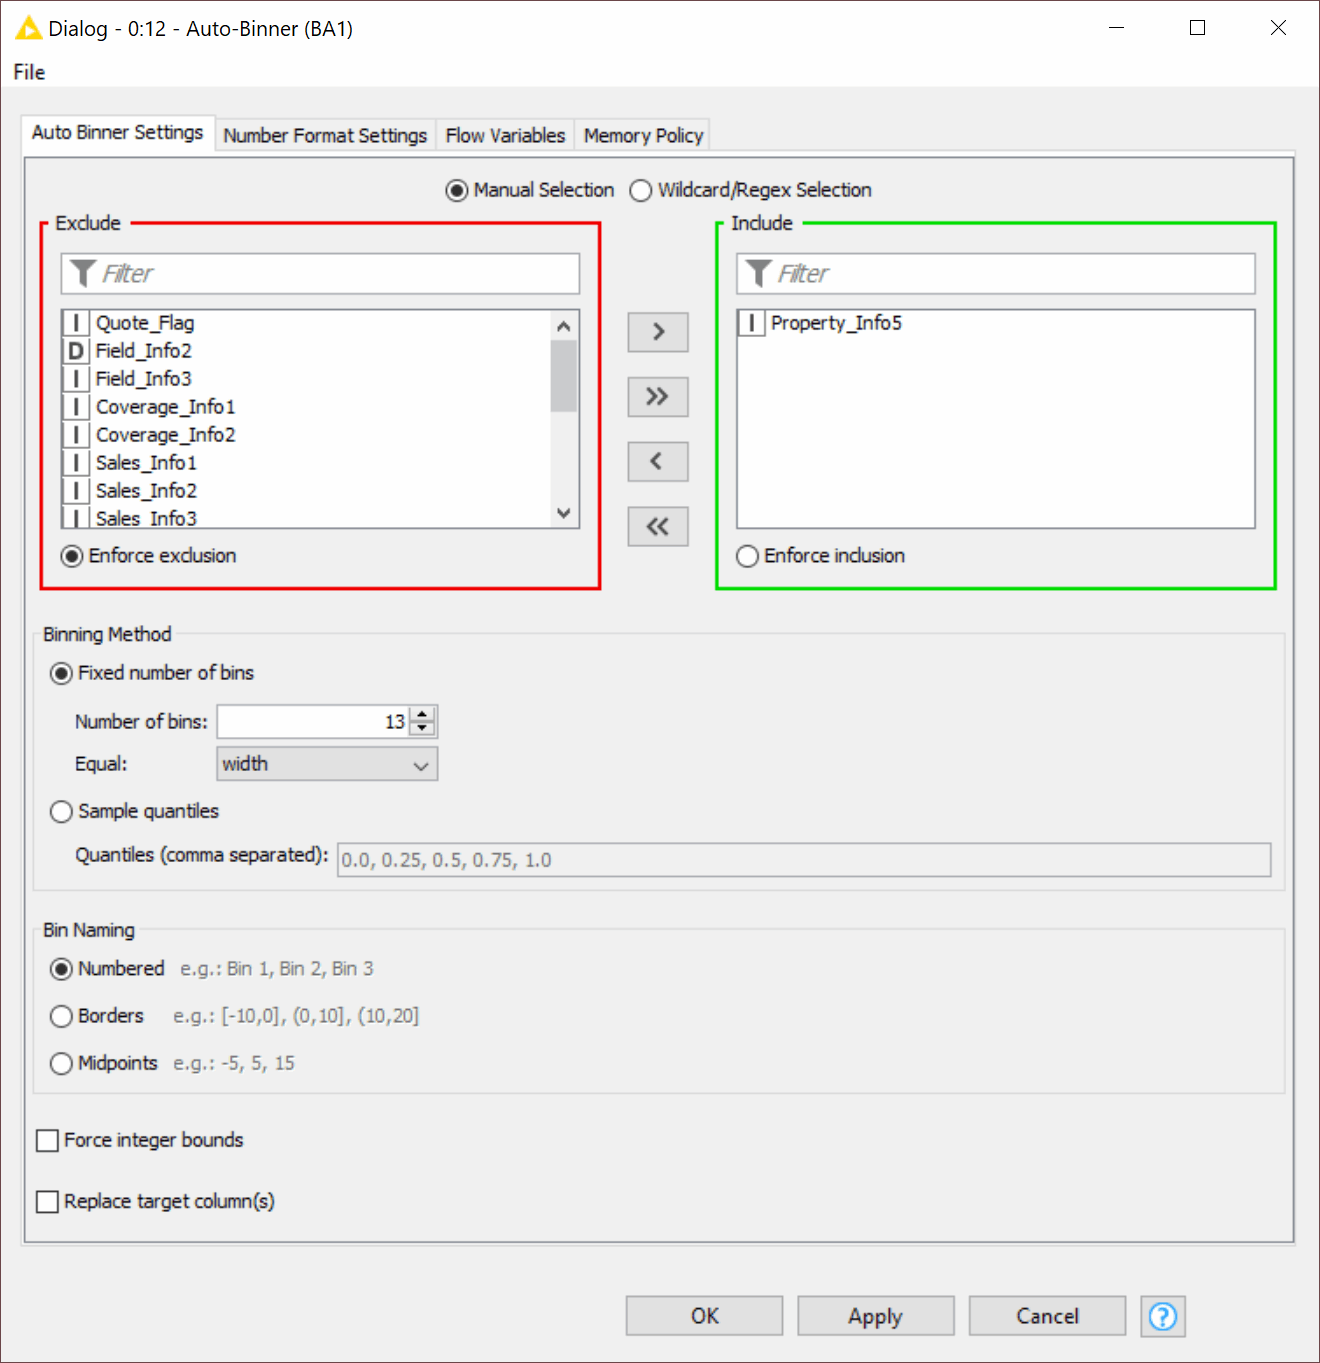
\includegraphics[width=0.4\textwidth]{Screen/Screen_Bin_1.png}
		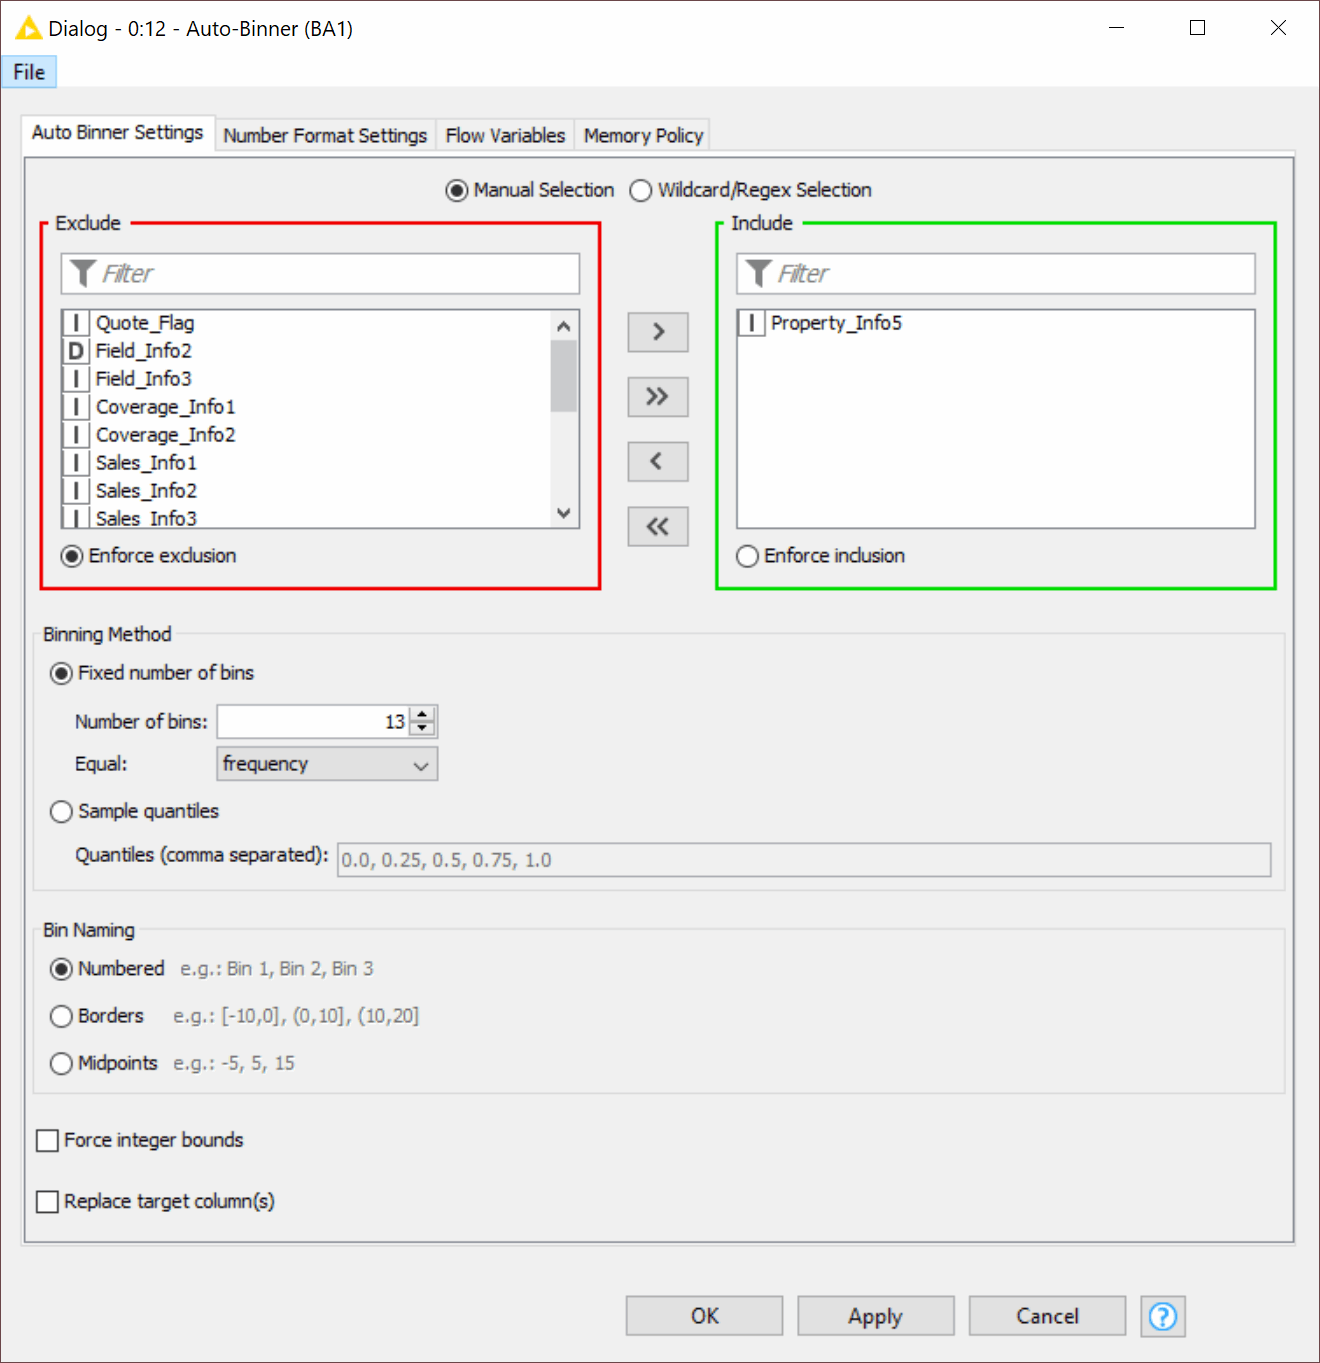
\includegraphics[width=0.4\textwidth]{Screen/Screen_Bin_2.png}
		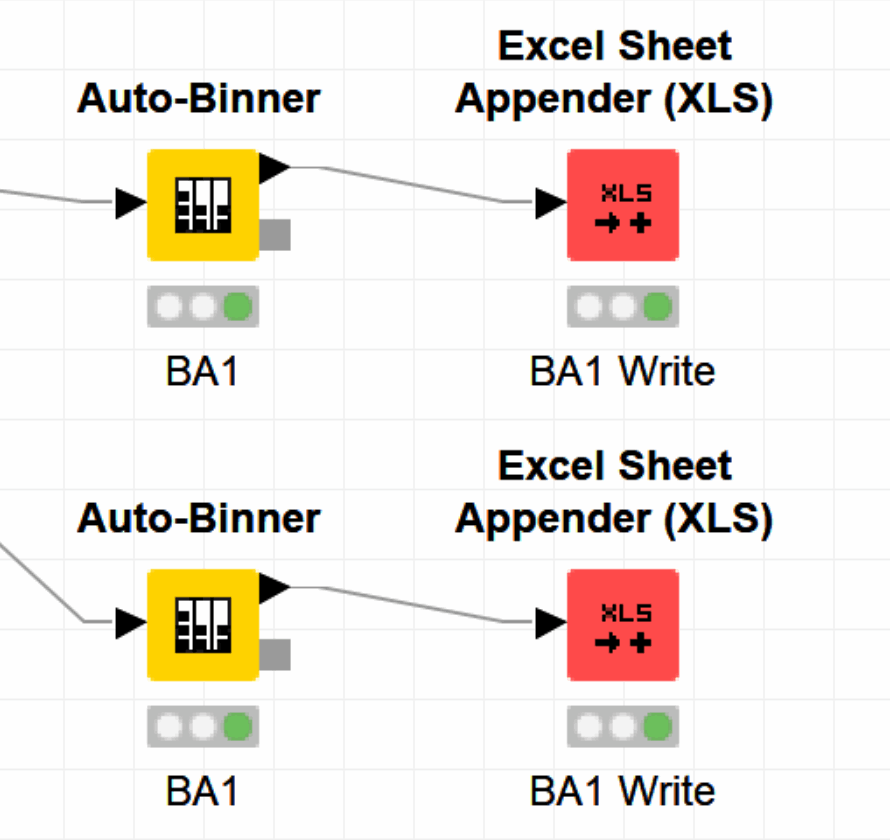
\includegraphics[width=0.4\textwidth]{Screen/Screen_Bin_3.png}
		
	\end{center}
	\caption{Screenshots Binning}
\end{figure}
\subsection{Normalization of Sales\_Info5}
\begin{figure}[H]
	\begin{center}
		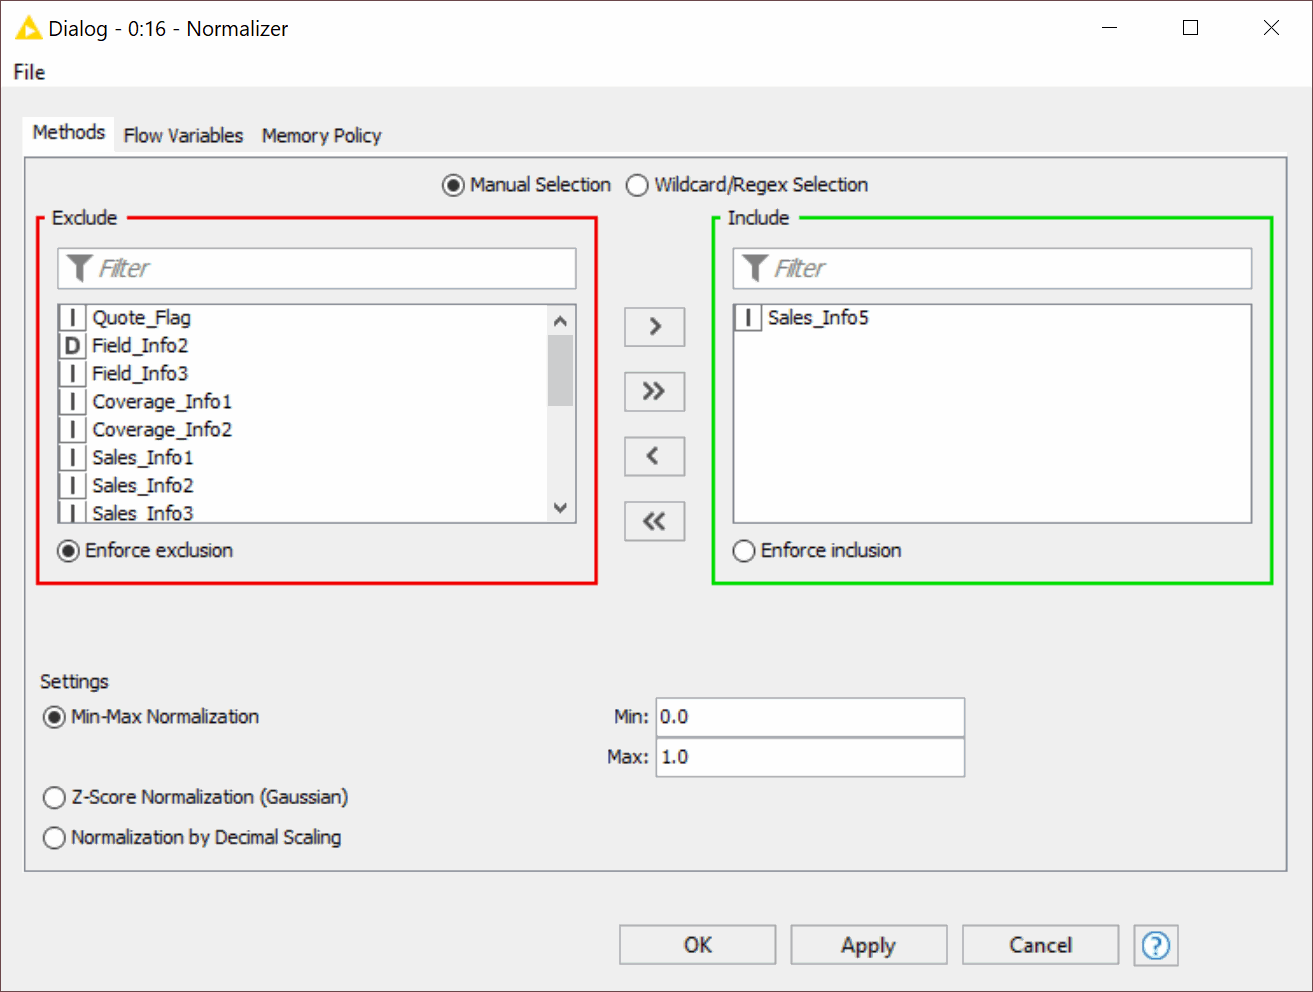
\includegraphics[width=0.4\textwidth]{Screen/Screen_Norm_1.png}
		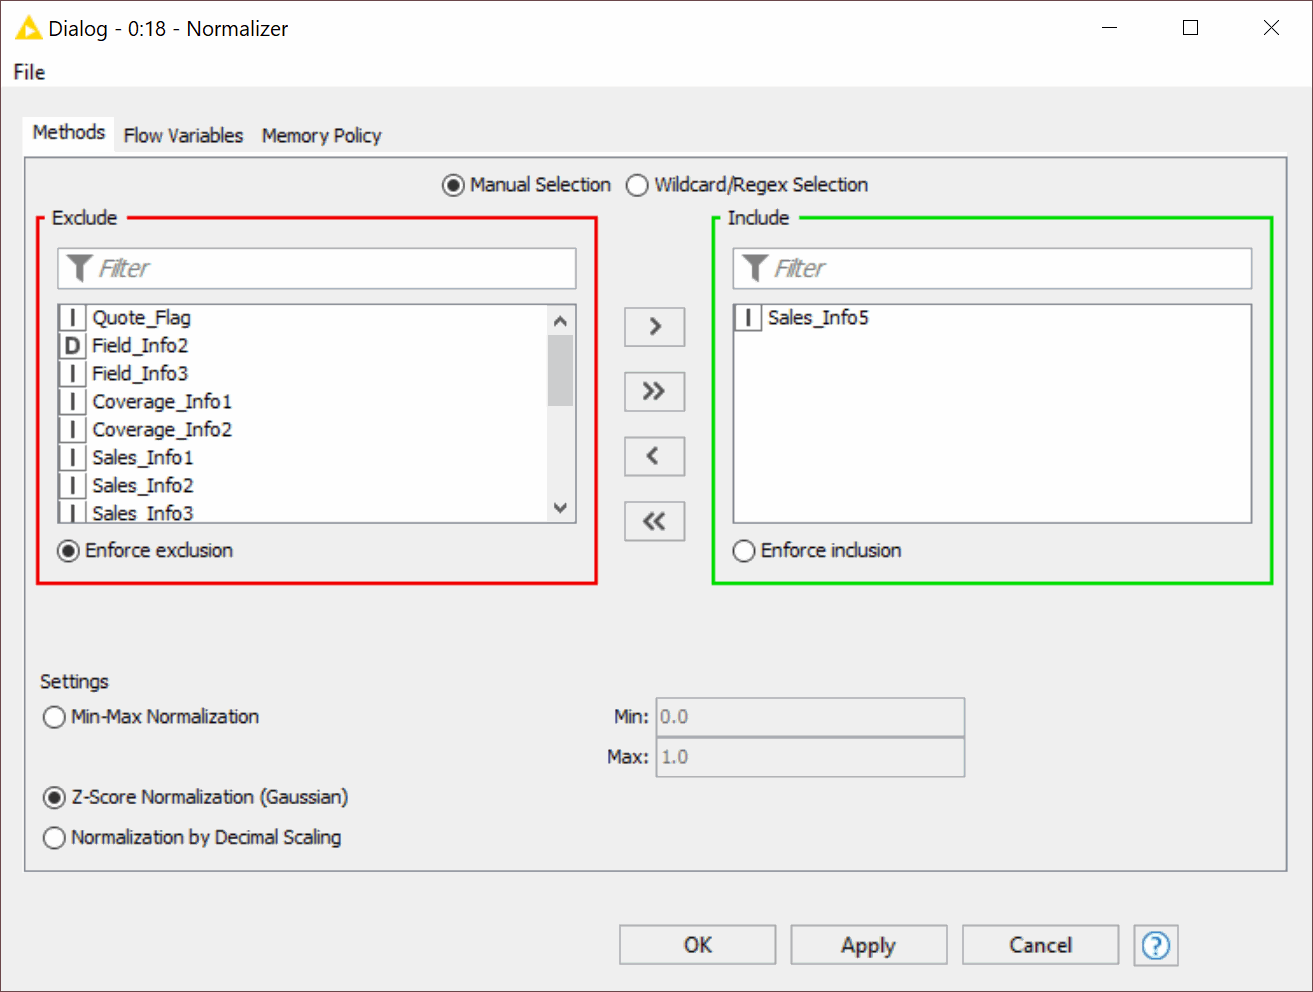
\includegraphics[width=0.4\textwidth]{Screen/Screen_Norm_2.png}
		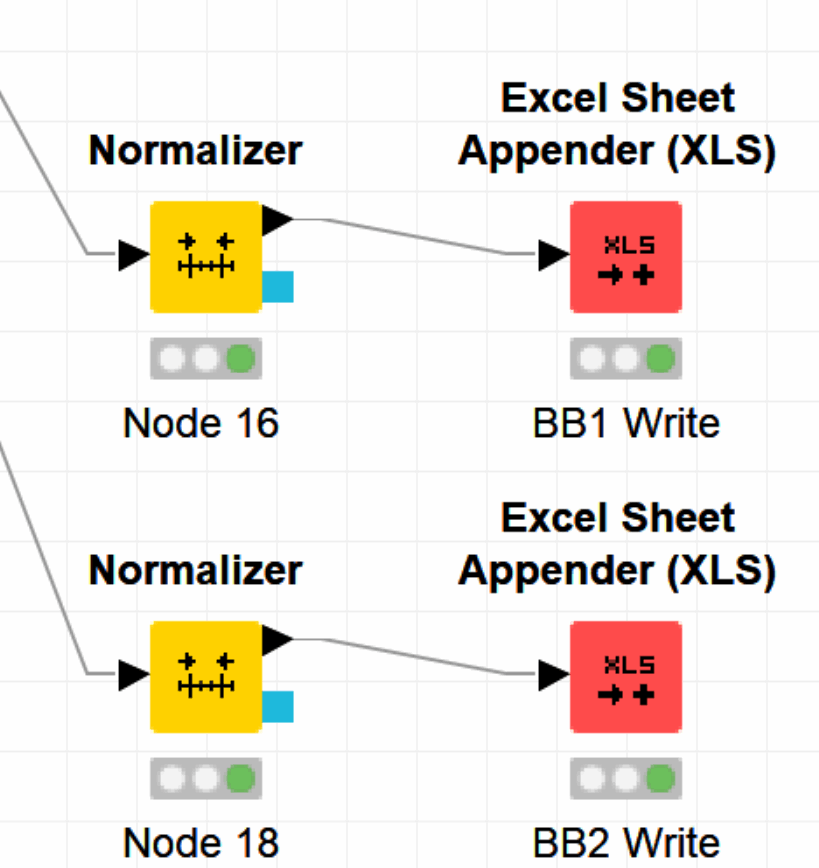
\includegraphics[width=0.4\textwidth]{Screen/Screen_Norm_3.png}
		
	\end{center}
	\caption{Screenshots Normalization}
\end{figure}
\subsection{Discretization of Coverage\_Info1}
Since the values in Coverage\_Info1 range from 1 to 25, it makes sense to set the range of each category to $6$ and the thresholds for the four categories as follows:
\begin{align*}
\text{Basic} &= ]-\infty , 7[\\
\text{Low} &= ]7 , 13[\\
\text{Medium} &= ]13 , 19[\\
\text{High} &= ]19 , \infty[
\end{align*}
\begin{figure}[H]
	\begin{center}
		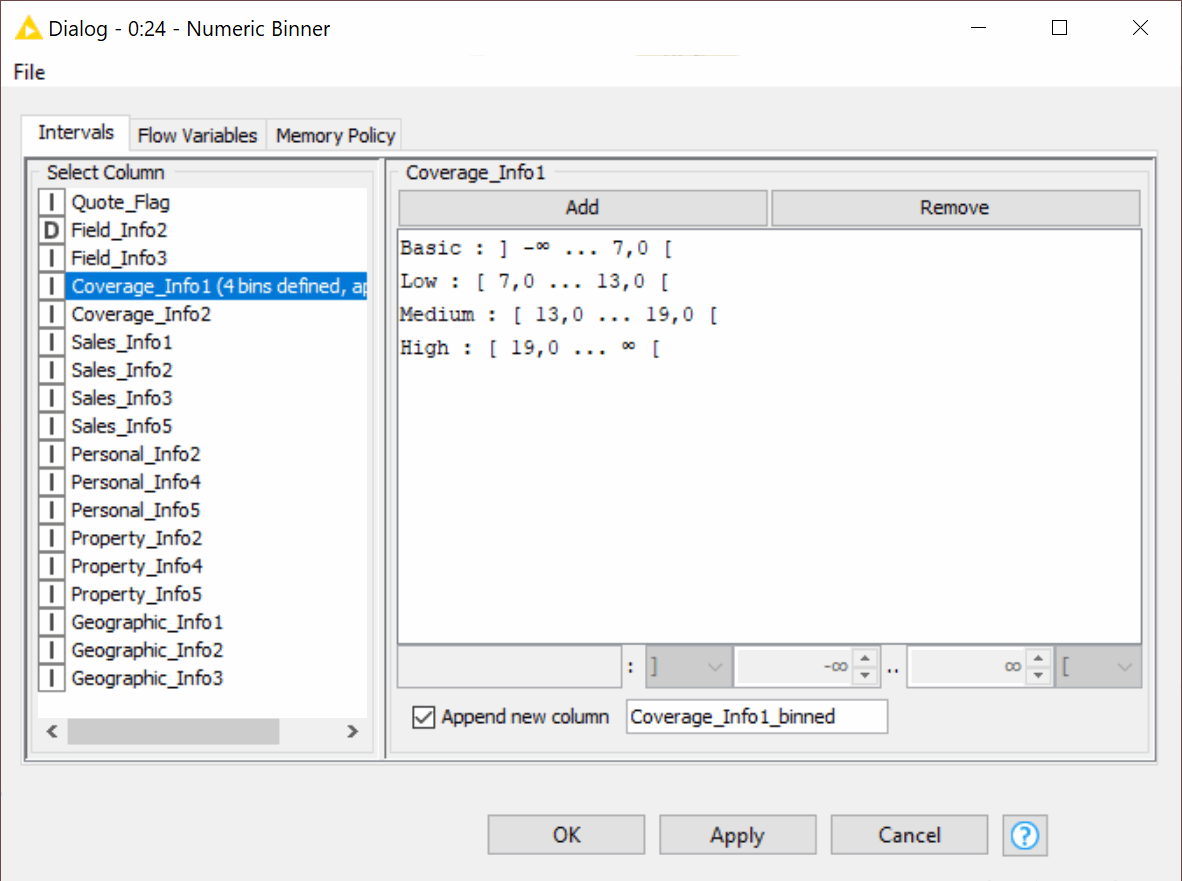
\includegraphics[width=0.8\textwidth]{Screen/Screen_Num_1.png}
		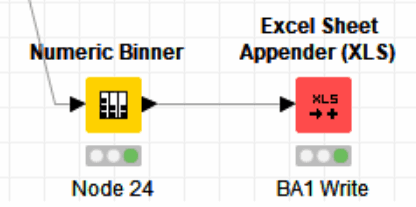
\includegraphics[width=0.5\textwidth]{Screen/Screen_Num_2.png}	
	\end{center}
	\caption{Screenshots Discretization}
\end{figure}
\subsection{Binarization of Geographic\_Info5}
To binarise the Attribute I used the "One to Many" Node in Knime. The result of the binarization can be found inside the attached excel-workbook.
\begin{figure}[H]
	\begin{center}
		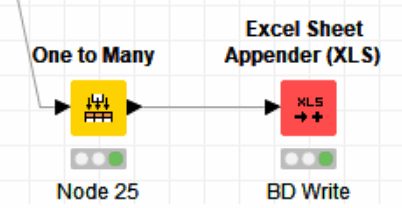
\includegraphics[width=0.4\textwidth]{Screen/Screen_Bina_1.png}
		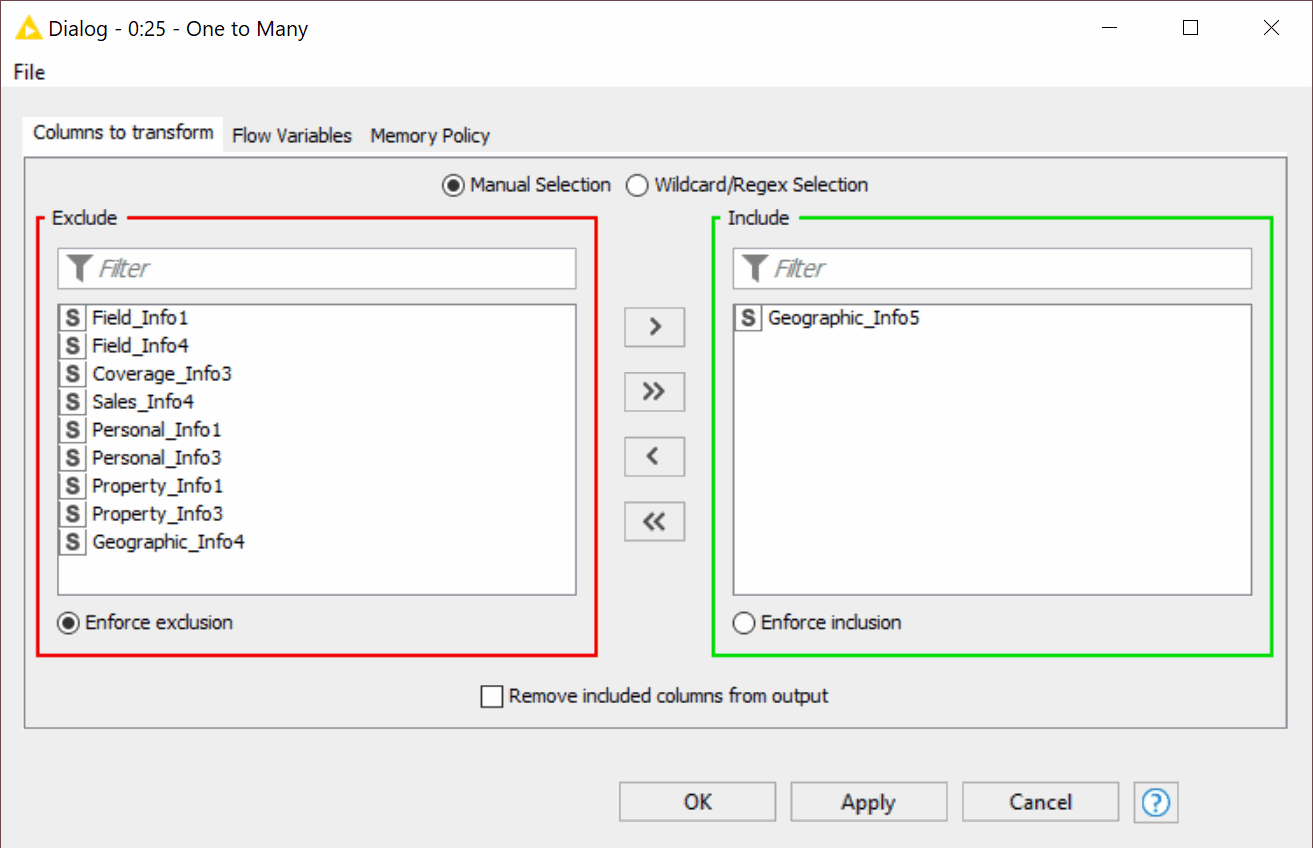
\includegraphics[width=0.4\textwidth]{Screen/Screen_Bina_2.png}
		
	\end{center}
	\caption{Screenshots Binarization}
\end{figure}
\section{Summary}

\paragraph{Field\_Info3} All values in this attribute are either on the side or in the middle of the range. 

\paragraph{Field\_Info4} Normal distribution, but there is a peak at the end.

\paragraph{Coverage\_Info2} On this attribute we only have datapoints with four different values allthough the range of those values suggets 25 options have been available.

\paragraph{Geographic\_Info2 \& Property\_Info 5} Both of these values show a  even distribution with a spike at the begin of their ranges.

\paragraph{Personal\_Info3} Almost $50 \text{\%}$ of the values are "ZA".
\paragraph{Property\_Info2} All values are $0$
\paragraph{Personal\_Info4} All values are $0$ except for one $1$

\subsubsection{Linear Correlations}

There are some interessting correlations in this dataset. Exspecially Geographic\_Info5 seems to have some strong correllations with Field\_Info2 and Coverage\_Info3. Field\_Info1 seems to be correlatted to Field\_Info4 and Field\_Info2 has as negative Correlation with Field\_Info3.






